\documentclass[journal]{IEEEtran}

\usepackage{subfigure}
\usepackage{setspace}
\usepackage{caption}  
\usepackage[english]{babel} 
\usepackage{amsfonts,amsmath,bm,bbm}
\usepackage{hyperref} 
\usepackage{graphicx,xurl}
\usepackage{rotating}
\usepackage{lipsum}
\usepackage{xcolor} 
\usepackage{tikz}
\usepackage{ifthen}
\usepackage{color}
\usepackage{multicol,multirow}
\usepackage{float}
\usepackage{siunitx}
\usepackage{algorithm,algorithmicx,algpseudocode}
\usepackage{booktabs}
\usepackage{scalerel}
\usepackage{tikz}
\usetikzlibrary{svg.path}

\definecolor{orcidlogocol}{HTML}{A6CE39}
\tikzset{
orcidlogo/.pic={
	\fill[orcidlogocol] svg{M256,128c0,70.7-57.3,128-128,128C57.3,256,0,198.7,0,128C0,57.3,57.3,0,128,0C198.7,0,256,57.3,256,128z};
	\fill[white] svg{M86.3,186.2H70.9V79.1h15.4v48.4V186.2z}
	svg{M108.9,79.1h41.6c39.6,0,57,28.3,57,53.6c0,27.5-21.5,53.6-56.8,53.6h-41.8V79.1z M124.3,172.4h24.5c34.9,0,42.9-26.5,42.9-39.7c0-21.5-13.7-39.7-43.7-39.7h-23.7V172.4z}
	svg{M88.7,56.8c0,5.5-4.5,10.1-10.1,10.1c-5.6,0-10.1-4.6-10.1-10.1c0-5.6,4.5-10.1,10.1-10.1C84.2,46.7,88.7,51.3,88.7,56.8z};
}
}

\newcommand\orcidicon[1]{\href{https://orcid.org/#1}{\mbox{\scalerel*{
			
\begin{tikzpicture}[yscale=-1,transform shape]
			\pic{orcidlogo};
			\end{tikzpicture}
		}{|}}}}


\renewcommand{\Bbb}{\mathbb}

% Author Orchid ID: enter ID or remove command
%\newcommand{\orcidauthorA}{0000-0001-9647-0506} 
%\newcommand{\orcidauthorB}{0000-0002-8002-5341} 
%\newcommand{\orcidauthorC}{0000-0002-1288-2528} 
%\newcommand{\orcidauthorD}{0000-0003-4523-6466}

\newdimen\HilbertLastX
\newdimen\HilbertLastY
\newcounter{HilbertOrder}

\def\DrawToNext#1#2{%
\advance \HilbertLastX by #1
\advance \HilbertLastY by #2
\pgfpathlineto{\pgfqpoint{\HilbertLastX}{\HilbertLastY}}
}

% \Hilbert[right_x,right_y,left_x,left_x,up_x,up_y,down_x,down_y]
\def\Hilbert[#1,#2,#3,#4,#5,#6,#7,#8] {
\ifnum\value{HilbertOrder} > 0%
\addtocounter{HilbertOrder}{-1}
\Hilbert[#5,#6,#7,#8,#1,#2,#3,#4]
\DrawToNext {#1} {#2}
\Hilbert[#1,#2,#3,#4,#5,#6,#7,#8]
\DrawToNext {#5} {#6}
\Hilbert[#1,#2,#3,#4,#5,#6,#7,#8]
\DrawToNext {#3} {#4}
\Hilbert[#7,#8,#5,#6,#3,#4,#1,#2]
\addtocounter{HilbertOrder}{1}
\fi
}

% \hilbert((x,y),order)
\def\hilbert((#1,#2),#3){%
\advance \HilbertLastX by #1
\advance \HilbertLastY by #2
\pgfpathmoveto{\pgfqpoint{\HilbertLastX}{\HilbertLastY}}
\setcounter{HilbertOrder}{#3}
\Hilbert[1mm,0mm,-1mm,0mm,0mm,1mm,0mm,-1mm]
\pgfusepath{stroke}%
}

% correct bad hyphenation here
\hyphenation{op-tical net-works semi-conduc-tor}


\begin{document}

\title{Analysis and Classification of SAR Textures using Information Theory}

\author{Eduarda~T.~C.~Chagas \orcidicon{0000-0001-9647-0506},
	Alejandro~C.~Frery \orcidicon{0000-0002-8002-5341},
	\IEEEmembership{IEEE~Senior~Member,}
	Osvaldo~A.~Rosso \orcidicon{0000-0002-1288-2528},
	and~Heitor~S.~Ramos \orcidicon{0000-0003-4523-6466},\IEEEmembership{IEEE~Senior~Member}
	
	\thanks{E.\ T.\ C.\ Chagas and H.\ S.\ Ramos ar with Departamento de Ci\^encia da Computa\c c\~ao, Universidade Federal de Minas Gerais, Belo Horizonte, Minas Gerais, Brazil (e-mail: eduarda.chagas@dcc.ufmg.br, ramosh@dcc.ufmg.br).}
	\thanks{A.\ C.\ Frery is with Laborat\'orio de Computa\c c\~ao Cient\'ifica e An\'alise Num\'erica -- LaCCAN, Universidade Federal de Alagoas, Brasil; (e-mail: acfrery@laccan.ufal.br)}
	\thanks{O.\ A.\ Rosso is with Instituto de F\'isica, Universidade Federal de Alagoas, Brasil (e-mail: oarosso@if.ufal.br)}
	\thanks{Manuscript received XX YY, 20ZZ; revised WW UU, 20VV.}}


\markboth{IEEE JOURNAL OF SELECTED TOPICS IN APPLIED EARTH OBSERVATIONS AND REMOTE SENSING}
%\markboth{IEEE JOURNAL OF SELECTED TOPICS IN APPLIED EARTH OBSERVATIONS AND REMOTE SENSING,~Vol.~13, No.~9, September~2014}%
{Shell \MakeLowercase{\textit{et al.}}: Bare Demo of IEEEtran.cls for Journals}

\maketitle

\begin{abstract}
	The use of Bandt-Pompe probability distributions and descriptors of Information Theory has been presenting satisfactory results with low computational cost in the time series analysis literature~\cite{Aquino2017Characterization, Rosso2016Signatures, Schieber2016network}.
	However, these tools have limitations when applied to data without time dependency.
	Given this context, we present a newly proposed technique for texture analysis and classification based on the Bandt-Pompe symbolization for SAR data.
	It consists of
	(i)~linearize a 2-D patch of the image using the Hilbert-Peano curve,
	(ii)~build an Ordinal Pattern Transition Graph that considers the data amplitude encoded into the weight of the edges;
	(iii)~obtain a probability distribution function derived from this graph;
	(iv)~compute Information Theory descriptors (Permutation Entropy and Statistical Complexity) from this distribution and use them as features to feed a classifier.
	The ordinal pattern graph we propose considers that the weight of the edges is related to the absolute difference of observations, which encodes the information about the data amplitude. 
	This modification takes into account the scattering properties of the target and leads to the characterization of several types of textures.
	Experiments with data from Munich urban areas, Guatemala forest regions and Cape Canaveral ocean samples show the effectiveness of our technique in homogeneous areas, which achieves satisfactory levels of separability.
	The two descriptors chosen in this work are easy and quick to calculate and are used as input for a k-nearest neighbor classifier.
	Experiments show that this technique presents results similar to state-of-the-art techniques that employ a much larger number of features and, consequently, require a higher computational cost.
\end{abstract}

\begin{IEEEkeywords}
	Synthetic Aperture Radar (SAR), 
	Texture, 
	Terrain Classification,		
	Permutation Entropy, 
	Ordinal Patterns Transition Graphs.
\end{IEEEkeywords}

\IEEEpeerreviewmaketitle

%\newpage
%\tableofcontents

\section{Introduction}

\IEEEPARstart{T}{exture} is an elusive trait.
When dealing with remotely sensed images, the texture of different patches carries relevant information that, more often than not, is hard to quantify and to transform into useful and parsimonious features.
This may be since textures, in this context, is a synesthesia phenomenon that triggers tactile responses from visual inputs.
This paper presents a new way of extracting features from textures, both natural and resulting from anthropic processes, in SAR (Synthetic Aperture Radar) imagery.

SAR systems are a vital source of data because they provide high-resolution images in almost all weather and day-night conditions.
They provide basilar information, complementary to that offered by sensors that operate in other regions of the electromagnetic spectrum, for a variety of Earth Observation applications.	
Although they present rich information, such data have challenging characteristics.
Most notably, they do not follow the usual Gaussian additive model, and the signal-to-noise ratio is usually low.

Yue et al.~\cite{Yue2020Gaussian} provide a comprehensive account of how the physical properties of the target are translated into first- and second-order statistical properties of SAR intensity data.
There is general agreement that non-deterministic textures are encoded in the second-order features, i.e., in the spatial correlation structure.
Therefore is frequent the use of covariance matrix and other measures that assume that a linear dependence, namely the Pearson correlation coefficient, suffices to characterize natural textures.
However, texture, in SAR imagery, is often visible only over large areas, and the multiplicative and non-Gaussian nature of speckle antagonizes with the additive assumption that underlies classical approaches, making complex the process of characterizing such data.

Surface classification and land use are among the most important applications of the Synthetic Aperture Radar (SAR) image~\cite{Pottier2004Unsupervised}.
In recent years, handcrafted features and representation learning (supervised and unsupervised) algorithms have been proposed~\cite{han2020unsupervised, huang2020classification, xie2020polsar}.
Algorithms of the unsupervised generative adversarial network (GAN) have revolutionized the classification of SAR images, improving performance in small sample problems, and helping the interpretability of such data~\cite{liu2019task}.
Among the supervised algorithms, support vector machine (SVM)~\cite{sukawattanavijit2017ga}, random forest (RF)~\cite{mcnairn2014early}, and neural network (NN)~\cite{lin2017deep} have been frequently used in remote sensing.
The Principle Component Analysis (PCA)~\cite{ressel2015neural}, autoencoder~\cite{wang2019classification} and the Boltzmann machine~\cite{qin2017object} can to extract non-local resources and classify non-labeled PolSAR pixels using an unsupervised approach.
However, methods such as graph-based semi-supervised deep learning algorithms~\cite{bi2018graph} can improve classification accuracy in problems with few labeled samples.

Handcrafted features in SAR textures can be studied following two complementary approaches, namely analyzing the marginal properties of the data (first-order statistics), and observing their spatial structure~\cite{Yue2020Gaussian, numbisi2018multi}.
In this work, we focus on the second approach, which has been showing relevant results using techniques from the image processing literature, such as co-occurrence matrices and Haralick's descriptors~\cite{yu2019detection}.
Through the GLCM we can extract features that reflect statistical relationships of the pixel intensity values.
On the other hand, Haralick's descriptors can capture information on intensity and amplitude based on global statistics of SAR images.
Radford et al.~\cite{radford2018geological} used textural information derived from gray-level co-occurrence matrices (GLCM), along with Random Forests, for geological mapping of remote and inaccessible localities; the authors obtained a classification accuracy of $\approx\SI{90}{\percent}$, even when using limited training data ($\approx\SI{0.15}{\percent}$ of the total data). 	
Hagensieker and Waske~\cite{hagensieker2018evaluation} evaluated the synergistic contribution of multi-temporal L-, C-, and X-band data to tropical land cover mapping, comparing classification outcomes of ALOS-2~\cite{kankaku2013alos}, RADARSAT-2~\cite{morena2004introduction}, and TerraSAR-X~\cite{breit2009terrasar} datasets for a study site in the Brazilian Amazon using a wrapper approach. 
The wrapper utilizes the gray-level co-occurrence matrix texture information and a  Random Forest classifier to estimate scene importance. 	
Storie~\cite{storie2018urban} proposed an open-source workflow for detecting and delineating the urban-rural boundary using Sentinel-1a SAR data.
The author used a combination of GLCM information and a k-means classifier to produce a three-category map that distinguishes urban from rural areas. 
In higher resolution image classification activities, it is necessary to obtain more granular information from the data by extracting local characteristics of the data, such as scale and orientation.
In this scenario, techniques such as Fourier power spectrum~\cite{Florindo2012Fractal}, random fields~\cite{zhu2016antarctic}, Gabor filter~\cite{dumitru2014information} and wavelet transform~\cite{akbarizadeh2012new} are usually applied.

In our approach, we opt to analyze the 1-D signals resulting from the linearization of the image samples, using non-parametric time series analysis techniques.
With this approach, we reduced the dimensionality of the data and map the spatial dependence of the pixels onto the temporal correlation used in such methods.
Next, we extract a probability distribution from the ordinal patterns of a new transition graph, herein proposed, which can discriminate different levels of amplitude, and we use well-known features borrowed from the Information Theory field to classify texture patches.

The main contribution of this work is the proposal of a new set of features for characterization and classification of SAR textures, based on a modification of the current ordinal patterns transition graph, incorporating relevant 1-D signal information.
Our proposal, hereinafter referred to as Weighted Amplitude Transition Graph (WATG), incorporates the absolute difference between the observations, weighting them in the calculation of the final value of their probabilities.
Experiments performed on homogeneous regions of SAR image textures indicate that this approach preserves essential information about the dynamics of the system, presenting excellent results in the classification of regions, where it has reached satisfactory levels of separability.
Since the proposed work has a low computational cost, the results obtained reveal that this technique has a great potential for incorporation in other applications, such as texture segmentation tools of SAR images.

The paper is structured as follows:
Section~\ref{methodology} describes our proposed methodology.
Section~\ref{linearization} presents the patch linearization process of the images.
In the Section~\ref{BP} we report the Bandt-Pompe symbolization process.
Section~\ref{OPTG} describes the ordinal patterns transition graphs.
Section~\ref{WATG} shows our technique of ordinal amplitude transition graph weighting by amplitudes.
In Section~\ref{HC} we report the Information Theory descriptors used throughout this work.
Section\~ref{Methods} we summarize the weighted ordinal patterns methods used to compare with our proposal.
Section~\ref{Results} describe the SAR image datasets, 
the analysis of ordinal pattern methods, 
experiments of sliding window selection, 
and a quantitative assessment.
Finally, Section~\ref{Conclusion} concludes the paper.

\section{Methodology}\label{methodology}

Algorithm~\ref{alg:watg} outlines our methodology.
%The main idea of the technique is as follows.
Line~\ref{Line:Peano} transforms theinput texture patch $P$ in a 1-D signal with a Hilbert-Peano sequence.
%
With this, the spatial information is encoded into a one-dimensional signal.
%
Line~\ref{Line:Probs} computes 
the probability distribution of the weighted transition graph induced by the 1-D signal.
The WATG function is detailed in Lines~\ref{Line:WATGBegin}--\ref{Line:WATGEnd}.
%
Lines~\ref{Line:Shannon} and~\ref{Line:StatisticalComplexity} compute the two descriptors of the patch.

The \texttt{WATG} function consists of three steps: 
(i)~each subsequence of size (dimension) $D$ of observations at delay $\tau$ is transformed into an ordinal pattern using the Bandt-Pompe symbolization (function \texttt{BPSymbolization}, Line~\ref{Line:BP}); 
(ii)~function \texttt{transitions} (Line~\ref{Line:Transitions}) calculates the sequence of alternations of the ordinal patterns; and 
(iii)~function \texttt{weigthGraph} (Line~\ref{Line:WG}) generates the incidence matrix of the graph using the as weights the amplitude differences between the time series elements.
Finally, the probability distribution is obtained by turning the transition matrix into a vector (Line~\ref{Line:WATGEnd}).

These steps are also depicted in Fig.~\ref{fig:WATG}, and are detailed in the following sections.

\begin{algorithm}[hbt]
	\caption{$H \times C$ point from a patch using WATG}
	\label{alg:watg}                                
	\textbf{Input:} Patch of texture $P$, dimension $D$ and time delay \textbf{$\tau$}\\
	\textbf{Output:} $H \times C$ feature
	\begin{algorithmic}[1]
		\State signal.1-D $\gets$ \texttt{hilbertCurve}($P$) \label{Line:Peano}
		\State Probs $\gets$ \texttt{WATG}(signal.1-D, D, $\tau$) \label{Line:Probs}
		\State H $\gets$ \texttt{ShannonEntropy}(Probs) \label{Line:Shannon}
		\State C $\gets$ \texttt{StatisticalComplexity}(Probs) \label{Line:StatisticalComplexity}
		
		\vspace{0.15cm}
		
		\Function{\texttt{WATG}}{signal.1-D, D, $\tau$}
		\State patterns $\gets$ \label{Line:WATGBegin} \texttt{BPSymbolization}(signal.1-D, D, $\tau$) \label{Line:BP}
		\State transitions $\gets$ \texttt{transitions}(patterns) \label{Line:Transitions}
		\State graph $\gets$ \texttt{weigthGraph}(signal.1-D, transitions) \label{Line:WG}
		\State Probs $\gets$ \texttt{as.vector}(graph) \label{Line:WATGEnd}
		\State \Return Probs
		\EndFunction
	\end{algorithmic}
\end{algorithm}


\begin{figure}[hbt]
	\centering
	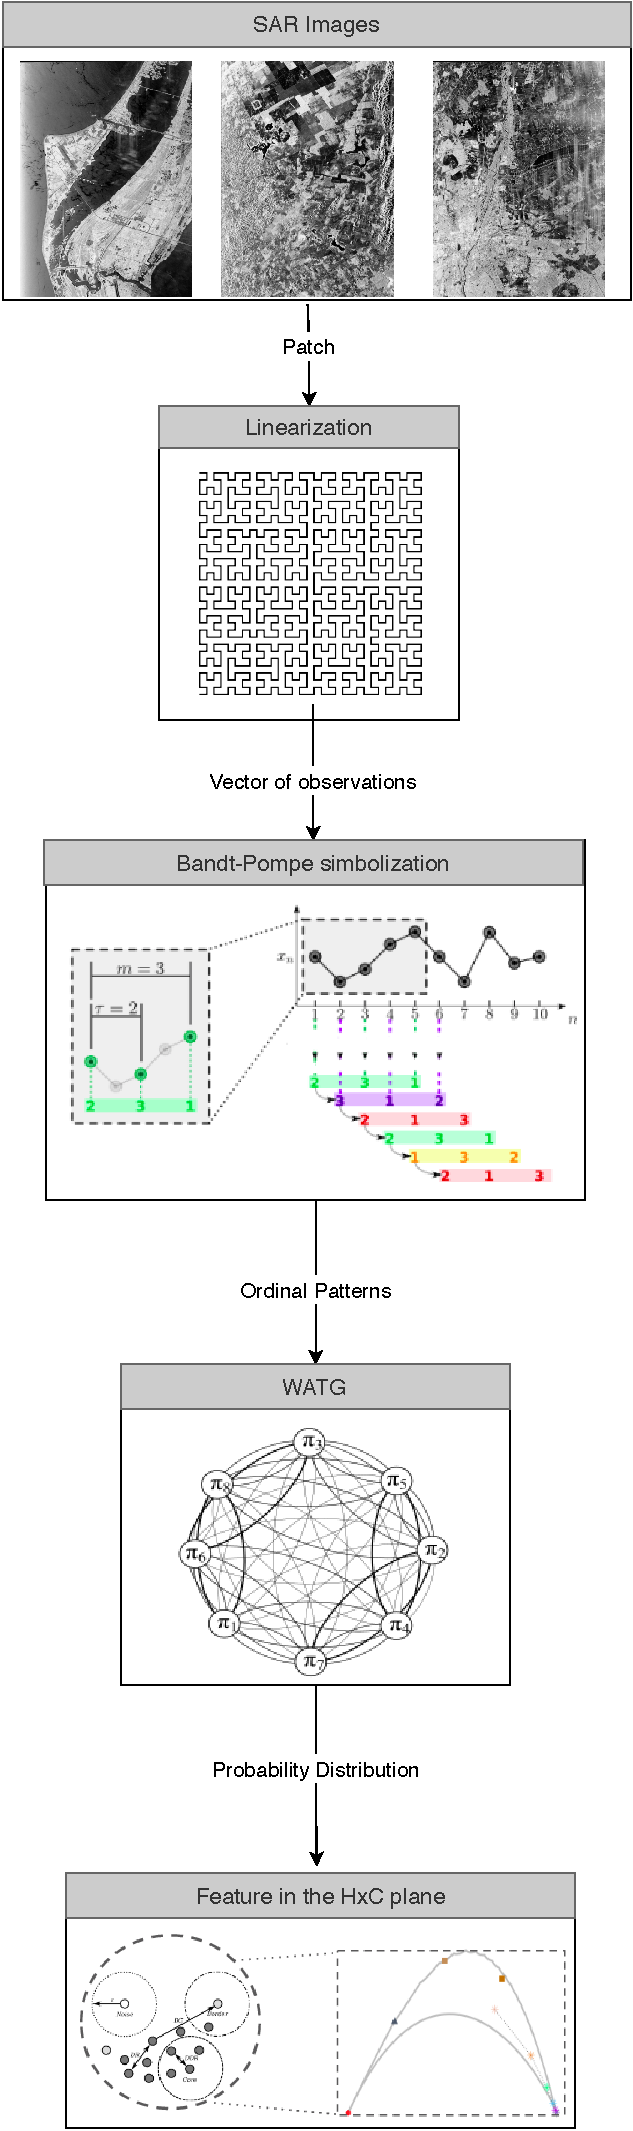
\includegraphics[width=.7\columnwidth]{Figures/methodology.pdf}
	\caption{Outline of the methodology used for the classification of textures.}
	\label{fig:WATG}
\end{figure}

\subsection{Linearization of image patches}\label{linearization}

In this step, we perform a data dimensionality reduction by turning the 2-D patch into a 1-D signal.
This could be accomplished by reading the data bylines, columns, or any transformation of 2-D indexes into a sequence of integers.
In this work, we chose to use the Hilbert-Peano~\cite{Lee1994Texture} curve, due to its low computational cost and its ability to preserve relevant properties of pixel spatial correlation.

Nguyen et al.~\cite{nguyen1982space} firstly employed Space-filling curves, to map texture into a one-dimensional signal.
%When used as scanning methods of an image, such functions preserve relevant properties of pixel spatial correlation~\cite{Lee1994Texture}.
Carincotte et al.~\cite{Carincotte2006changeDetection} used the Hilbert-Peano curve in the problem of change detection in pairs of SAR images.
The authors noted that this transformation exploits the spatial locality and that its pseudo-randomness
of direction changes works well for a large family of images, especially
natural ones.

Assuming an image patch is supported by an $M \times N$ grid, we have the following definition.

\newtheorem{mydef}{Definition}
\begin{mydef}
	An image scan is a bijective function $f \colon \mathbb{N} \times \mathbb{N} \to \mathbb{N}$ in the ordered pair set $ \{(i, j): 1 \leq i \leq M , 1 \leq j \leq N\}$, which denotes the points in the domain, for the closed range of integers $\{1, \dots, M  N\}$.
	A scan rule is $\{f^{-1}(1), \dots, f^{-1}(M  N)\}$.
	\label{def:CurveFilling}
\end{mydef}
This Definition imposes that each pixel is visited only once, and that all pixels are visited.

Space-filling curves, such as raster-1, raster-2, and Hilbert-Peano scanning techniques, stipulate a proper function $f$.
Traditional Hilbert-Peano curves scan an array of pixels of dimension $2^k \times 2^k$, $k \in \mathbb{N}$, never keeping the same direction for more than three consecutive points, as shown in Fig.~\ref{fig:Hilbert}.
Using the Hilbert-Peano curve, we reduce the data dimensionality by maintaining the spatial dependence information of the patch.
In this work, we use Hilbert-Peano patches of size $128 \times 128$.

\begin{figure}[hbt]
	\centering
	\tikz[scale=3.2] \hilbert((0mm,0mm),3);
	\hspace{0.3cm}
	\tikz[scale=1.5] \hilbert((0mm,0mm),4);
	\hspace{0.3cm}
	\tikz[scale=0.73] \hilbert((0mm,0mm),5);	
	\caption{Visual representation of Hilbert-Peano curve in areas of: (a) $8 \times 8$, (b) $16 \times 16$ and (c) $32 \times 32$. }\label{fig:Hilbert}
\end{figure} 

\subsection{Bandt-Pompe Symbolization}\label{BP}

%Step~\ref{item:WOPTG} consists of two stages.
%In the first, the time series is transformed into a sequence of ordinal patterns.
%In the second, we build a weighted graph describing the transitions between these patterns.

The representation of time series by ordinal patterns was introduced by Bandt and Pompe~\cite{Bandt2002Permutation} as a transformation resistant to noise, and invariant to nonlinear monotonic transformations.
Therefore, the first step of the \texttt{WATG} subroutine is to calculate the ordinal patterns of the 1-D signal by Band-Pompe symbolization.

Consider ${\mathcal X} \equiv \{x_t\}_{t=1}^{T}$ a real valued time series of length $T$. 
Let ${\mathfrak A}_{D}$ (with $D \geq 2$ and $D \in {\Bbb N}$) be the symmetric group of order $D!$ formed by all 
possible permutation of order $D$, and the symbol component vector 
${\bm \pi}^{(D)} = (\pi_1, \pi_2, \dots, \pi_D)$ so every element ${\bm \pi}^{(D)}$ is unique 
($\pi_j \neq \pi_k$ for every $j \neq k$). 
Consider for the time series ${\mathcal X} \equiv \{x_t\}_{t=1}^{T}$ its time delay embedding representation,
with embedding dimension $D \geq 2$ and time delay $\tau \geq 1$ ($\tau \in {\Bbb N}$, also called ``embedding time,'' ``time delay'', or ``delay''):
\begin{equation} 
\label{eq:time-delay}
{\mathbf X}^{(D,\tau)}_t =( x_t,x_{t+\tau},\dots,x_{t+(D-1)\tau} ) ,
\end{equation} 
for $t = 1,2,\dots,N$ with $N = T-(D-1) \tau$.
Then the vector ${\mathbf X}^{(D,\tau)}_t$ can be mapped to a symbol vector ${\bm \pi}_t^D \in {\mathfrak A}_{D}$. 
This mapping is such that preserves the desired relation between the elements 
$x_t  \in {\mathbf X}^{(D,\tau)}_t$, and all $t \in \{1,\dots,T-(D-1)\tau\}$ that share this pattern (also called ``motif'') have to be mapped to the same 
${\bm \pi}_t^{D}$.

We define the mapping ${\mathbf X}_t^{(D,\tau)} \mapsto {\mathbf \pi}_t^{D}$ by ordering the observations $x_t \in {\mathbf X}_t^{(D,\tau)}$ in increasing order.
Consider the time series $\mathcal X = (1.8, 1.2, 3.2, 4.8, 4.2, 4.5, 2.3, 3.7, 1.2, .5)$ depicted in Fig.~\ref{Fig:IntroBP}.
Assume we are using patterns of length $D=5$ with unitary time lag $\tau=1$.
The code associated to $\mathbf X_{3}^{(5,1)}=(x_3,\dots,x_7)=(3.2, 4.8, 4.2, 4.5, 2.3)$, shown in black, is formed by the indexes in $\bm\pi_3^{5}=(1,2,3,4,5)$ which sort the elements of $\mathbf X_{3}^{(5,1)}$ in increasing order: $51342$.
With this, $\widetilde{\pi}_3^{5} = 51342$, and we increase the counting related to this motif in the histogram of all possible patterns of size $D=5$.

The dash-dot line in Fig.~\ref{Fig:IntroBP} illustrates $\mathbf X_{1}^{(5,2)}$, i.e. the sequence of length $D=5$ starting at $x_1$ with lag $\tau=2$.
In this case, $\mathbf X_{1}^{(5,2)}= (1.8, 3.2, 4.2, 2.3, 1.2)$, and the corresponding motif is $\widetilde{\pi}_1^{5}=51423$.

\begin{figure}[hbt]
	\centering
	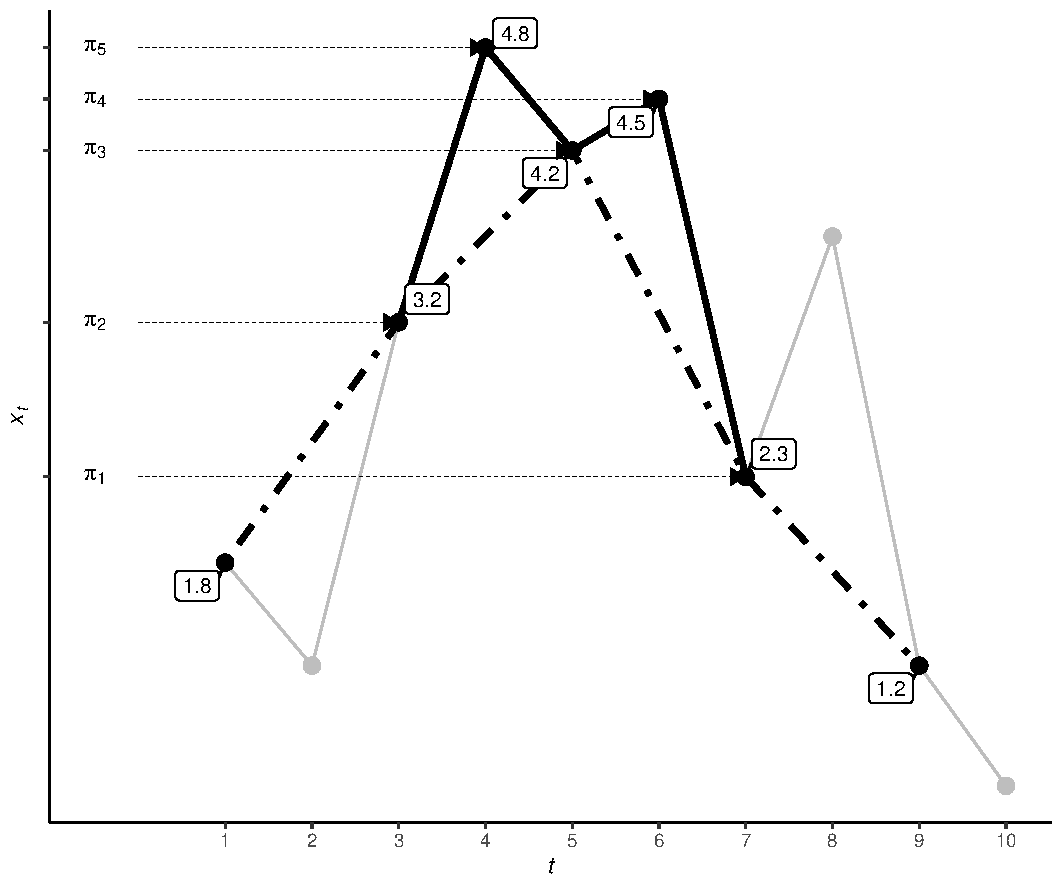
\includegraphics[width=.9\linewidth]{Figures/IntroBP.pdf}
	\caption{Illustration of the Bandt and Pompe coding\label{Fig:IntroBP}}
\end{figure}

The classic approach to calculating the probability distribution of ordinal patterns is through the frequency histogram.
Denote $\Pi$ the sequence of symbols obtained by a given series $\mathbf{X}_t^{(D,\tau)}$.
The Bandt-Pompe probability distribution is the relative frequency of symbols in the series against the $D!$ possible patterns $\{\widetilde\pi_t^D \}_{t = 1}^{D!}$:
\begin{equation}
p(\widetilde\pi_t^D) = \frac{\#\left \{\mathbf{X}_t^{(D,\tau)} \text{ is of type } \widetilde\pi_t^D\right \}}{T- (D-1)\tau},  
\end{equation}
where  $t\in \{1, \dots, T-(D-1)\tau\}$.
These probabilities meet the conditions $p(\widetilde\pi_t^D) \ge 0$ and  $\sum_{i=1}^{D!} p(\widetilde\pi_t^D) = 1$, and are invariant before monotonic transformations of the time series values.

\subsection{Ordinal Pattern Transition Graph}\label{OPTG}

Alternatively, one may form an oriented graph with the transitions from $\widetilde\pi_t^D$ to $\widetilde\pi_{t+1}^D$. 
The Ordinal Pattern Transition Graph ${G} = ({V}, {E})$ 
represents the transitions between two consecutive ordinal patterns over time $t$.
The vertices are the patterns, and the edges the transitions between them:
$V = \{v_{\widetilde\pi_t^D}\}$, and 
$E = \{(v_{\widetilde\pi_t^D}, v_{\widetilde\pi_{t+1}^D}): v_{\widetilde\pi_t^D}, v_{\widetilde\pi_{t+1}^D} \in V \}$~\cite{Borges2019Transition}.

The literature reports two approaches to compute the weight of edges.
Some authors employ unweighted edges~\cite{McCullough2015lagged,Kulp2016ordinal} which represent only the existence of transitions, while others apply the frequency of transitions~\cite{Sorrentino2015periodic,Zhang2017ConstructingOP}.
The weights $\mathbb{W} = \{w_{v_{\widetilde{\pi}^D_i}, v_{\widetilde\pi^D_j}}: v_{\widetilde\pi^D_i}, v_{\widetilde\pi^D_j} \in V \}$ assigned to each edge describe the chance of transitions between the patterns $(v_{\widetilde\pi^D_i}, v_{\widetilde\pi^D_j})$
The weights are calculated as the relative frequency of each transition, i.e., as:
\begin{equation}
w_{v_{\widetilde\pi^D_i}, v_{\widetilde\pi^D_j}} = \frac{|\Pi_{\widetilde\pi^D_i,\widetilde\pi^D_j}|}{T-(D-1)\tau-1},
\end{equation}
where $|\Pi_{\widetilde\pi^D_i,\widetilde\pi^D_j}|$ is the number of transitions from pattern $\widetilde\pi^D_i$ to pattern $\widetilde\pi^D_j$, $\sum_{v_{\widetilde\pi^D_i}, v_{\widetilde\pi^D_j}}w_{v_{\widetilde\pi^D_i}, v_{\widetilde\pi^D_j}} = 1$,
and the denominator is the number of transitions between sequential patterns in the series of motifs of length $T-(D-1)\tau$.

\subsection{Weighted Ordinal Patterns Methods}\label{Methods}

Recent works proposed using weights in the calculation of relative frequencies for ordinal patterns.
They all aim at incorporating the information coded in the amplitude of the observations back into the Permutation Entropy.
We summarize in the following those that we used for comparison with our proposal.

\subsubsection{Weighted Permutation Entropy}\label{WPE}

The Weighted Permutation Entropy (WPE) was proposed by Fadlallah et al.~\cite{Fadlallah2013Weightedpermutation}. 

Denote $\overline{X}_t^{(D, \tau)}$ the arithmetic mean:
\begin{equation}
\overline{X}_t^{(D, \tau)} = \frac{1}{D} \sum_{k = 1}^{D} x_{t + (k - 1)}.
\end{equation}
The weight $w_{t}$ is the sample variance of each vector $X_t^{(D, \tau)}$:
\begin{equation}
w_{t} = \frac{1}{D} \sum_{k = 1}^{D}\big[x_{t + (k - 1)} - \overline{X}_t^{(D, \tau)}\big]^2 .
\end{equation}
Then, the probability distribution is given from the weighted relative frequencies:
\begin{equation}
p(\widetilde \pi_t^D) = \frac{\sum_{i : \{\mathbf{X}^{(D,\tau)}_i \mapsto \widetilde\pi^D_t\}} w_{i}}{\sum_{i = 1}^{T-(D-1)\tau} w_{i}}.
\end{equation}

\subsubsection{Fine-Grained Permutation Entropy}\label{FGPE}

The Fine-Grained Permutation Entropy (FGPE) was introduced in Ref.~\cite{xiao2009fine}.

Let $\beta_t$ be the difference series:
\begin{equation}
\beta_t = \big\{|x_{t+1} - x_t|, \dots, |x_{t+(D-1)} - x_{t+(D-2)}|\big\}.
\end{equation}
The weight $w_t$ quantifies such differences:
\begin{equation}
w_t = \left \lfloor \frac{\max\{\beta_t\}}{\alpha s(\beta_t) } \right \rfloor,
\end{equation}
where $s$ is the sample standard deviation,
$\alpha$ is a user-defined parameter, 
and $\lfloor \rfloor$ is the floor function.
Then, $w_t$ is added as a symbol at the end of the corresponding pattern, leading to an update of $\Pi$:
\begin{equation}
\pi{'}_t^D = \{ \widetilde \pi_t^D \cup w_t\}.
\end{equation} 
Finally, the probability distribution is calculated as:
\begin{equation}
p(\pi{'}_t^D) = \frac{\#\left \{\mathbf{X}_t^{(D,\tau)} \text{ is of type } \pi{'}_t^D\right \}}{T- (D-1)\tau}.
\end{equation}

\subsubsection{Amplitude-Aware Permutation Entropy}\label{AAPE}

The Amplitude-Aware Permutation Entropy (AAPE) was proposed in Ref.~\cite{azami2016amplitude}.
It consists of weighting the amplitude of ordinal patterns by both the mean and the differences of the elements.
For this, only an additional parameter $ A \in [0, 1]$ is required, being:
\begin{equation}
w_t = \frac{A \cdot |x_t|}{D} + \sum_{k = 1}^{D - 1} \left(\frac{A \cdot |x_{t + k}|}{D} + \frac{(1 - A) \cdot |x_{t+k} - x_{t+k-1}|}{D - 1}\right)
\end{equation}
The probability distribution is given from the weighted relative frequencies:
\begin{equation}
p(\widetilde \pi_t^D) = \frac{\sum_{i : \{\mathbf{X}^{(D,\tau)}_i \mapsto \widetilde\pi^D_t\}} w_{i}}{\sum_{i = 1}^{T-(D-1)\tau} w_{i}}.
\end{equation}

\subsection{Weighted Ordinal Patterns Transition Graph}\label{WATG}

Our proposal for computing the probability distribution, henceforth referred to as Weighted Amplitude Transition Graph (WATG), takes into account the dispersion intensity of the target's backscatter, leading to a good characterization of the textures.
We propose a modification of the current ordinal pattern transition graph, incorporating the absolute difference between the observations that produced the patterns.

First, each $\mathcal{X}$ time series is scaled to $[0, 1]$, since we are interested in a metric able to compare datasets:
\begin{equation}
\frac{x_i - x_{\min}}{x_{\max} - x_{\min}} \longmapsto x_i,
\end{equation}
where $x_{\min}$ and $x_{\max}$ are, respectively, the minimum and maximum values of the series.
This transformation is relatively stable before contamination, e.g., if instead of $x_{\max}$ we observe $k x_{\max}$ with $k\geq 1$, the relative values are not altered. Nevertheless, other more resistant transformations as, for instance, $z$ scores, might be considered.

Each $\mathbf{X}^{(D, \tau)}_t$ vector is associated with a weight $\beta_t$ that measures the largest difference between its elements:
\begin{equation}
\beta_t = \max\{x_i - x_j\},
\end{equation}
where $x_i, x_j \in \mathbf{X}^{(D, \tau)}_t$.

We propose that the weight assigned to each edge is proportional to the amplitude difference observed in the transition:	
\begin{equation}
w_{v_{\widetilde \pi^D_i}, v_{\widetilde \pi^D_j}} =  \sum_{i : \{\mathbf{X}^{(D,\tau)}_t \mapsto \widetilde\pi^D_i\}} \sum_{j : \{\mathbf{X}^{(D,\tau)}_t \mapsto \widetilde\pi^D_j\}} |\beta_i - \beta_j| .
\end{equation}
Thus, the probability distribution taken from the weighted amplitude transition graph is given as follows:	
\begin{align}
&\left\{\begin{array}{l}
\lambda_{v_{\widetilde\pi^D_i}, v_{\widetilde\pi^D_j}} = 1, \text{ if } (v_{\widetilde\pi^D_i}, v_{\widetilde\pi^D_j}) \in {E}, \\
\lambda_{v_{\widetilde\pi^D_i}, v_{\widetilde\pi^D_j}} = 0, \text{ otherwise}.
\end{array}\right., \text{ and} \\
&p(\widetilde\pi^D_i, \widetilde\pi^D_j) = \frac{\lambda_{v_{\widetilde\pi^D_i}, v_{\widetilde\pi^D_j}} \cdot w_{v_{\widetilde\pi^D_i}, v_{\widetilde\pi^D_j}}}{\sum_{v_{\widetilde\pi^D_a}, v_{\widetilde\pi^D_b}} w_{v_{\widetilde\pi^D_a}, v_{\widetilde\pi^D_b}}}.
\end{align}

Note that the conditions $p(\widetilde\pi^D_i, \widetilde\pi^D_j) \ge 0$ and $\sum_{\widetilde\pi^D_i, \widetilde\pi^D_j} p(\widetilde\pi^D_i, \widetilde\pi^D_j) = 1$ are satisfied.

Thus, series with uniform amplitudes have edges with probability of occurrence well distributed along the graph, while those with large peaks have edges with probability of occurrence much higher than the others.

\subsection{Information-Theoretic Descriptors}\label{HC}

We chose two Information Theory descriptors: Shannon Entropy and Statistical Complexity.
Computing these quantities is the last step of the algorithm, i.e., obtaining the point in the $H \times C$ plane.

Entropy measures the disorder or unpredictability of a system characterized by a probability measure $\mathbb{P}$.
Let $\mathbb{P} = \{p_{(\widetilde\pi^D_1, \widetilde\pi^D_1)}, p_{(\widetilde\pi^D_1, \widetilde\pi^D_2)}, \dots, p_{(\widetilde\pi^D_{D!}, \widetilde\pi^D_{D!})} \} = \{p_1,\dots,p_{D!^2}\}$ be the probability function obtained from the 1-D signal weighted amplitude transition graph $\mathbb{X}$.
Its normalized Shannon entropy is given by:	
\begin{equation}
H(\mathbb{P}) = -\frac1{2\log D!}\sum_{\ell=1}^{D!^2} p_{\ell} \log p_{\ell} .
\label{eq:Entropia}
\end{equation}

The ability of the entropy to capture system properties is limited, so it is necessary to use it in conjunction with other des\-criptors to obtain a more complete analysis.
Other interesting measures are the distances between $\mathbb{P}$ and a probability measure that describes a non-informative process, typically the uniform distribution.

The Jensen-Shannon distance to the uniform distribution $\mathbb{U} = (\frac{1}{D!^2}, \dots, \frac{1}{D!^2})$ is a measure of how similar the underlying dynamics is to a non-informative process.
It is calculated as:
\begin{equation}
Q'(\mathbb{P}, \mathbb{U}) = \sum_{\ell=1}^{D!^2} \Big(p_\ell \log\frac{p_\ell}{u_\ell} +
u_\ell \log\frac{u_\ell}{p_\ell}
\Big).
\end{equation}
This quantity is also called ``disequilibrium.''
The normalized disequilibrium is $ Q=Q'/\max\{Q'\}$.

Conversely to entropy, the statistical complexity seeks to find interaction and dependence structures among the elements of a given series, being an extremely important factor in the study of dynamic systems.
The Statistical Complexity is then defined as~\cite{Lamberti2004Entropic}:
\begin{equation}
C(\mathbb{P}, \mathbb{U}) = H(\mathbb{P}) Q(\mathbb{P}, \mathbb{U}).
\end{equation}

In our analysis, each time series can then be described by a point $(H(\mathbb{P}), C(\mathbb{P}, \mathbb{U}))$.
The set of all pairs $(H(\mathbb{P}), C(\mathbb{P}, \mathbb{U}))$ for any time series described by patterns of length $D$ lies in a compact subset of $\mathbbm R^2$: the Entropy-Complexity plane.
Mart\'{\i}n et al~\cite{martin2006generalized} obtained explicit expressions for the boundaries of this closed manifold, which depend only on the dimension of the probability space considered, that is, $D!$ for the traditional Bandt-Pompe method and our case $D! \times D!$.
Through such a tool it is possible to discover the nature of the series, determining if it corresponds to a chaotic (or other deterministic dynamics) or stochastic sequences

\subsection{Properties}

To analyze the properties of WATG, we carried out two experiments to assess your response to different noise levels and image rotations.
For this, we use a deterministic image generated by the following function $z$:
\begin{equation*}
 z \sim \sin (4x + 0.5y), 
\end{equation*}
where  $x, y \in [-2\pi, 2\pi]$.
The present speckle noise, however, was modeled as:
\begin{equation*}
 speckle(l) \sim \Gamma(\alpha = l, \beta = l),
\end{equation*}
with $l \in \{1, 100, 150, 200, 250, 300, 350, 400, 450, 500\}$.
Thus, the $I(l)$ images were formed by:
\begin{equation*}
 I(l) = z \times speckle,
\end{equation*}
The robustness analysis in image rotations was performed using $I(l)^T$, which corresponds to the $I$ transpose.
Examples of the different images generated can be seen in Fig.~\ref{fig:speckle}.

\begin{figure}[hbt]
	\begin{tabular}{ccc}
		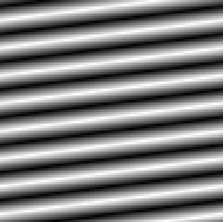
\includegraphics[width=0.135\textwidth]{Figures/z.png} &   
		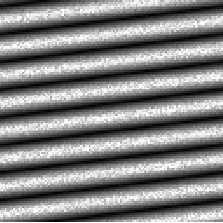
\includegraphics[width=0.135\textwidth]{Figures/z100.png} &
		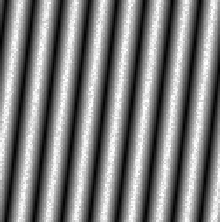
\includegraphics[width=0.135\textwidth]{Figures/z500t.png} \\
		(a) $z$ &   
		(b) $I(100)$ &
		(c) $I^T(500)$ \\
	\end{tabular}
	\caption{Visual representation of the data used in the robustness experiment.}
	\label{fig:speckle}
\end{figure}

As a result, we were able to verify that the higher $I$, the less noisy the pixels become, and we can see the in Fig.~\Ref{fig:speckleHC} that the statistical complexity and permutation entropy of the associated texture will be lower.
On the other hand, we observe that the features are slightly sensitive to rotation, presenting variations in the order of magnitude of only 4 decimal places, thus maintaining the order of the position of the samples in the $H \times C$ plane.

\begin{figure}[hbt]
	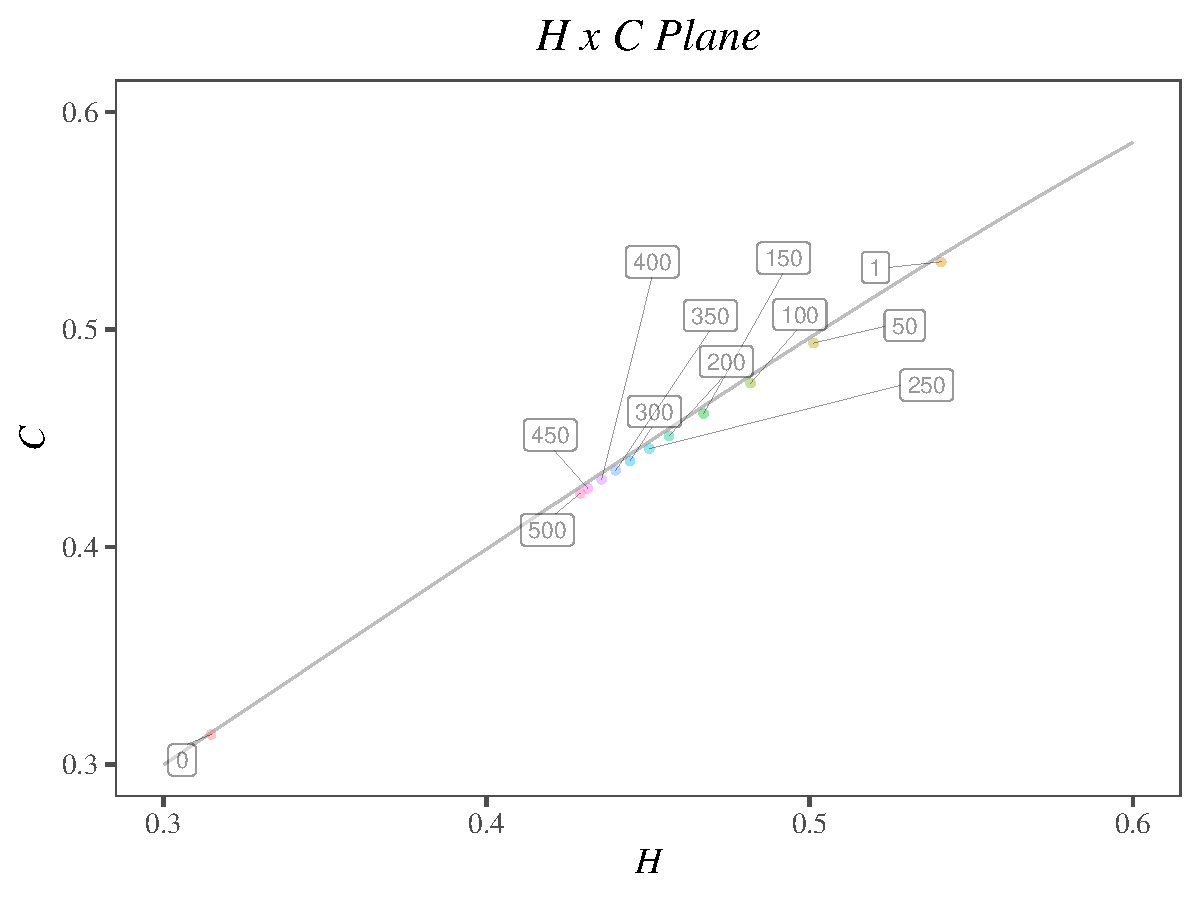
\includegraphics[width=0.45\textwidth]{Figures/waves1.pdf}
	\caption{Modifications to the $H \times C$ Plane features by adding different multiplicative noises.}
	\label{fig:speckleHC}
\end{figure}

\section{EXPERIMENTAL RESULTS AND ANALYSIS}\label{Results}

In this section, we describe the dataset, 
the classification process, and 
the results of the experiments.
To assess the performance of the technique here proposed, we first analyze the impact of its parameters and then compare its results in the classification with other methods.

\subsection{Image Dataset}

The proposed method was evaluated by dataset based on three quad-polarimetric L-band SAR images from the NASA Jet Propulsion Laboratory’s (JPL’s) uninhabited aerial vehicle synthetic aperture radar (UAVSAR) with $\sim 2$m range resolution and $36$ looks.
We used the HH backscatter magnitudes of:
\begin{itemize}
	\item Sierra del Lacandón National Park, forest region in Guatemala (acquired on April 10, 2015)\footnote{\protect{\url{https://uavsar.jpl.nasa.gov/cgi-bin/product.pl?jobName=Lacand_30202_15043_006_150410_L090_CX_01\#dados}}}. 
	It was $8917 \times 3300$ pixels and its image resolution is $10$m $\times 2$m;
	\item Cape Canaveral Ocean Regions (acquired on September 22, 2016).
	It was $7038 \times 3300$ pixels and its image resolution is $10$m $\times 2$m;
	\item Urban area of the city of Munich, Germany (acquired on June 5, 2015)\footnote{\protect{\url{https://uavsar.jpl.nasa.gov/cgi-bin/product.pl?jobName=munich_19417_15088_002_150605_L090_CX_01\#data}}}.
	It was $5773 \times 3300$ pixels and its image resolution is $10$m $\times 3$m.
\end{itemize}

We manually selected $200$ samples of size $128 \times 128$ to compose the dataset used in the experiments.
It is organized as follows:
$40$ samples from Guatemalan forest regions;
$40$ samples from Guatemalan pasture regions;
$80$ samples from the oceanic regions of Cape Canaveral, divided into two types with different contrast; and
$40$ samples of urban regions of the city of Munich.
Fig.~\ref{fig:samples} shows examples of each.

%In the classification, to avoid overlapping between samples and to preserve the general distribution of the classes, the training, test and validation data were determined based on a random sampling carried out in each region of analysis.
We randomly split the samples in training (\SI{85}{\percent}) and test (\SI{15}{\percent}) sets.
We used the first set to train a $k$-nearest neighbor classifier algorithm with tenfold cross-validation.
%The test samples were not used in the training stage.

\subsection{Analysis of ordinal patterns methods}

Fig.~\ref{fig:timeSeries} shows examples of the ocean, forest, urban, and pasture samples as sequences values, after the linearization process.
Data resulting from remote sensing have a peculiar feature that justifies the application in this article:
The variation in the magnitude of the targets' backscatter and, consequently, in the intensity of the image pixels, depends on the intrinsic properties of the regions under analysis.
Urban targets usually exhibit the strongest variation, followed by pasture, forests, and finally, water bodies.
By adding information related to amplitude, the proposed method is able to increase, compared to traditional methods, the granularity of information captured by ordinal patterns.
Fig.~\ref{fig:plotsHC} shows the evolution of the descriptive power of these techniques.

The Bandt-Pompe symbolization was the first method based on ordinal patterns proposed in the literature.
As shown in Fig.~\ref{fig:plotsHC} left, it provides a limited separation of the textures.
Transition graphs (Fig.~\ref{fig:plotsHC} center) improve the spread of the features, but with some amount of confusion.
Our proposal, shown in Fig.~\ref{fig:plotsHC} right, produces well-separated features.
%When considering the dynamics of alternating between consecutive patterns in a sequence, the transition graphs provide more information about the reference target and, consequently, this method is able to differentiate most of these dynamics, but there are challenging situations without a clear separation between them, causing misclassifications.
%On the other hand, as discussed in the section~\ref{WATG}, the weighted graph provides greater weight for transitions between ordinal patterns that have a wide range of amplitude.
%While in the traditional graph, the weight of the edges was obtained only by the frequency of the transitions, in the proposed method the symbols that appear with the same frequency gain different importance.
In this way, we were able to obtain, for this experiment, a perfect characterization and, consequently, the high descriptive power of the regions.
%In addition, some edges may disappear if the variation in amplitude between ordinal patterns is zero.

\begin{figure*}[hbt]
	\begin{tabular}{ccccc}
		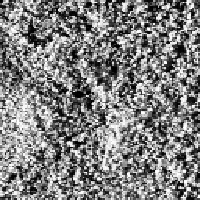
\includegraphics[width=0.175\textwidth]{Figures/guatemalaflorest.pdf} &   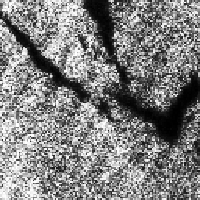
\includegraphics[width=0.175\textwidth]{Figures/Cape1.pdf} &
		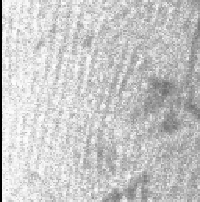
\includegraphics[width=0.175\textwidth]{Figures/Cape2.pdf} &  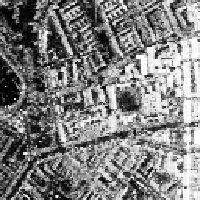
\includegraphics[width=0.175\textwidth]{Figures/munichUrban.pdf} &  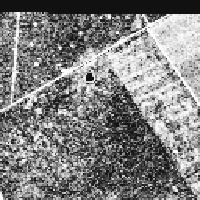
\includegraphics[width=0.175\textwidth]{Figures/pasture.pdf} \\
	\end{tabular}
	\caption{Types of regions analyzed: Guatemala forest, Canaveral ocean type 1, ocean type 2, Munich urban area, and pasture area.}
	\label{fig:samples}
\end{figure*}

\begin{figure*}[hbt]
	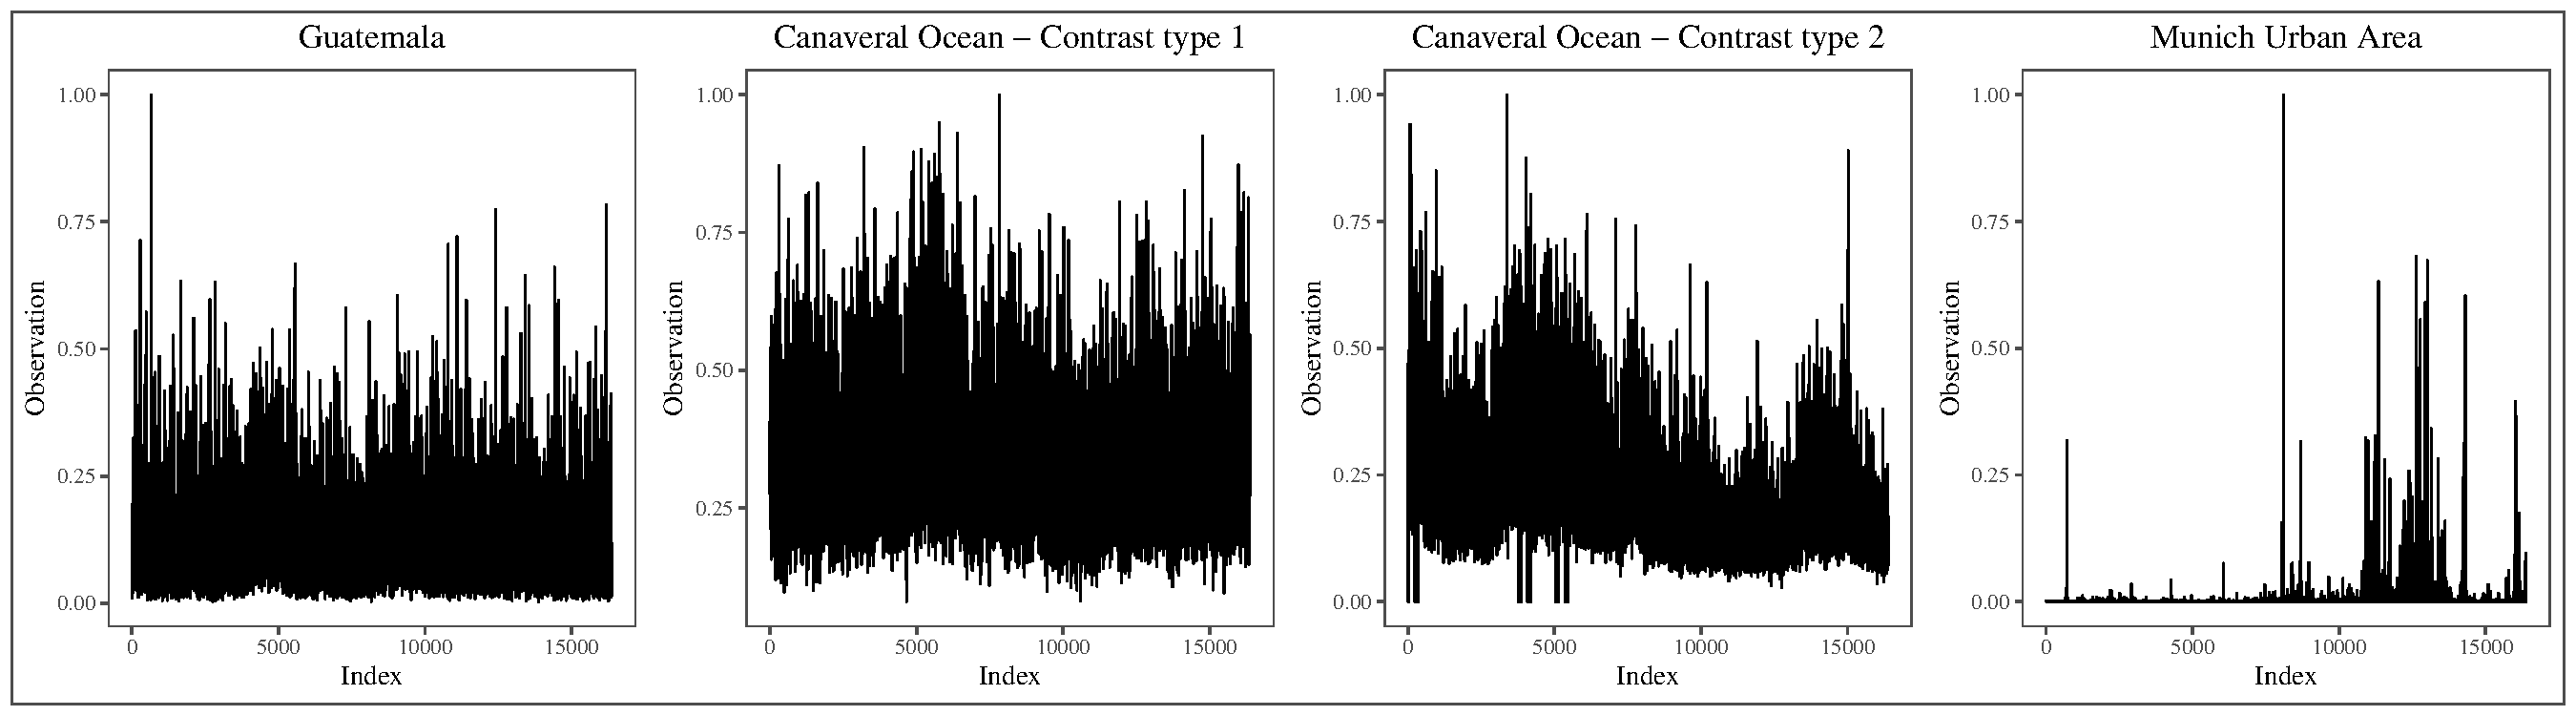
\includegraphics[width=2\columnwidth]{Figures/SAR_TS.pdf}
	\caption{Amplitude of different types of regions}
	\label{fig:timeSeries}
\end{figure*}

\begin{figure*}[hbt]
	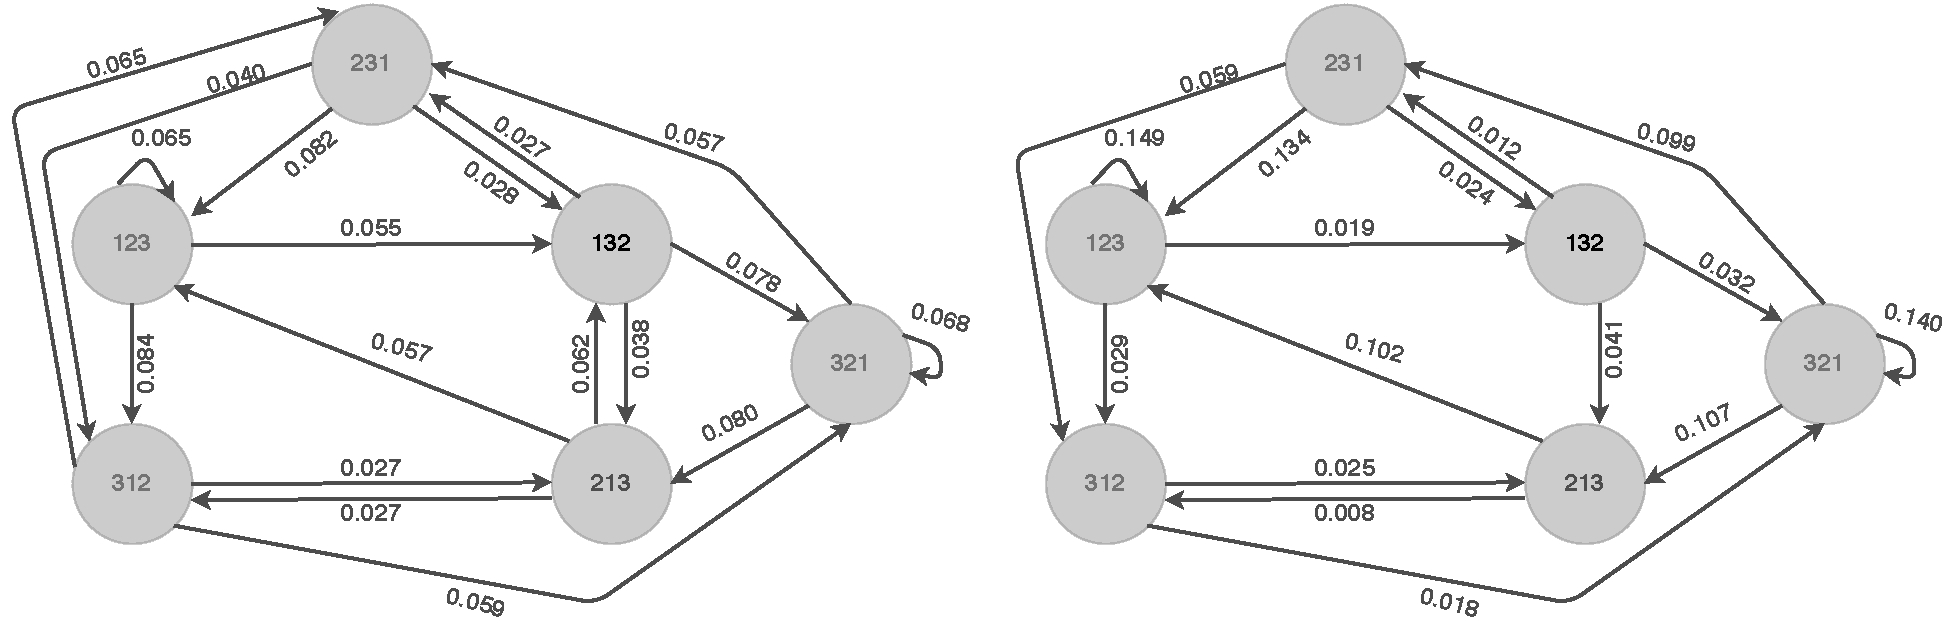
\includegraphics[width=2\columnwidth]{Figures/graphs.pdf}
	\caption{Example of the difference in weights at the edges in a sample of Munich urban regions in the transition graph and in the weighted graph of ordinal patterns
		transition to dimension 3 and delay 1}
	\label{fig:graphs}
\end{figure*}

\begin{figure*}[hbt]
	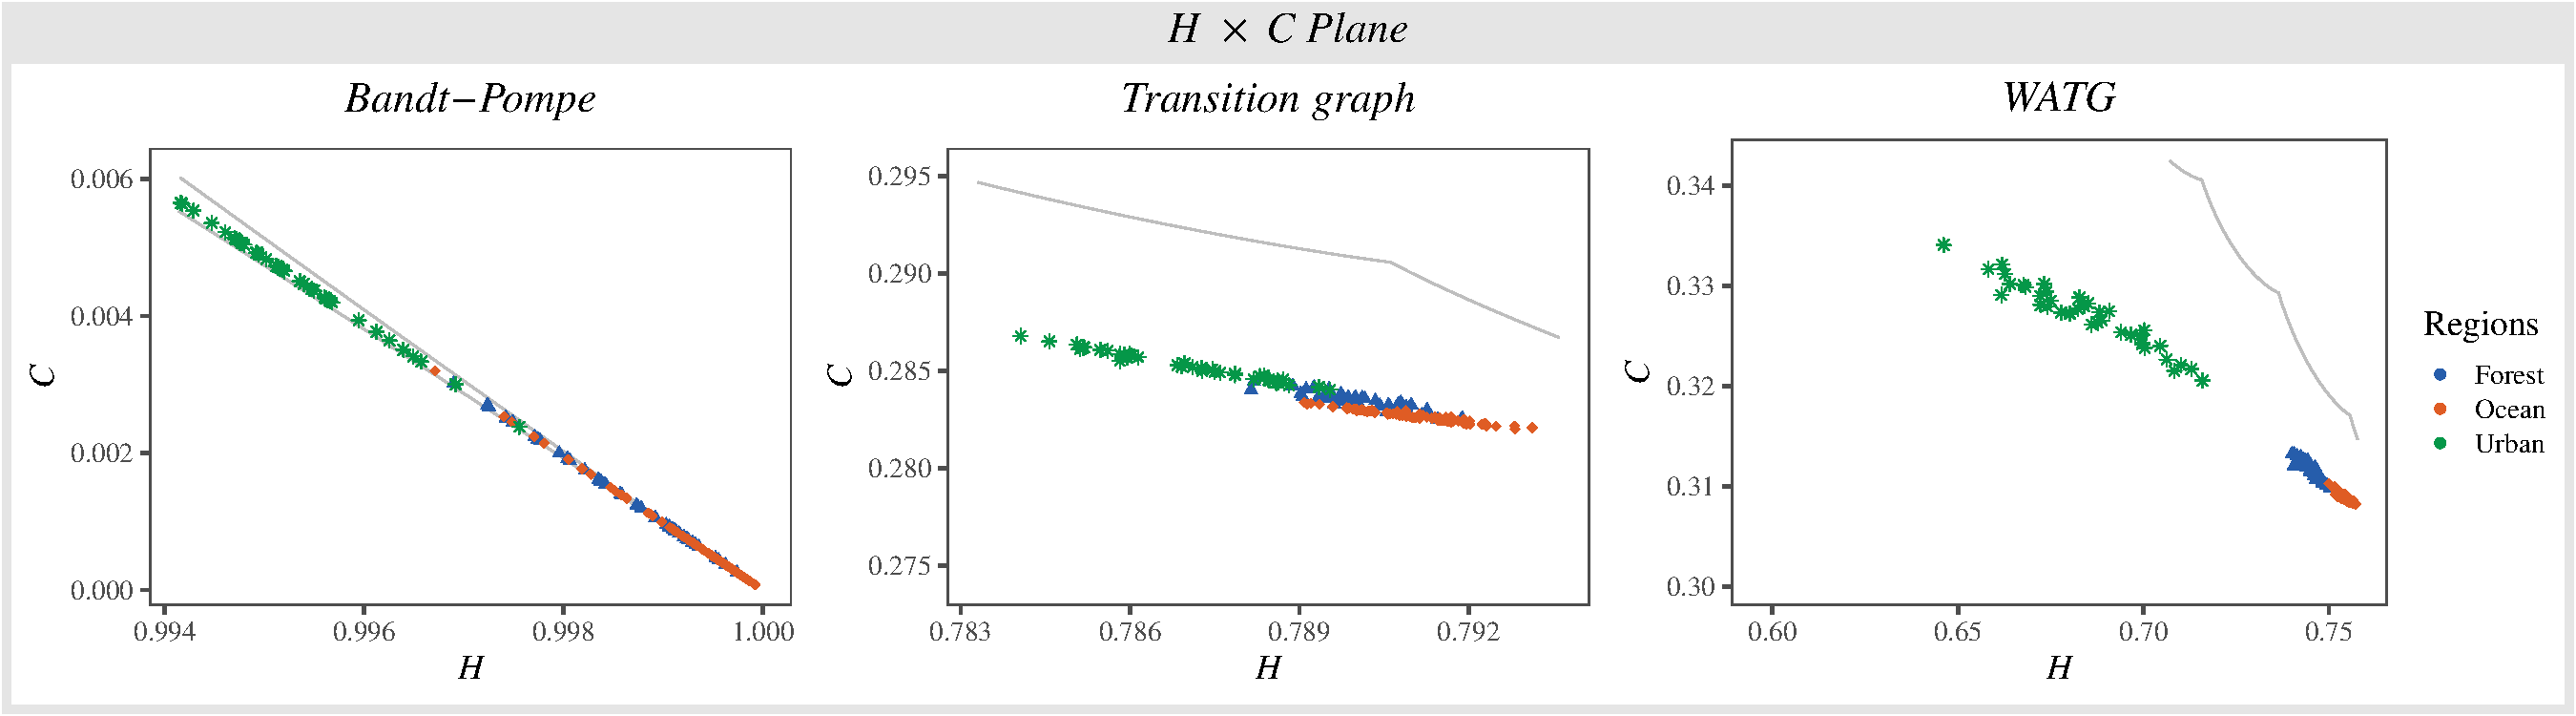
\includegraphics[width=2\columnwidth]{Figures/HCAnalysis.pdf}
	\caption{Location of Guatemala (forest), Cape Canaveral (ocean), and Munich (urban) in the $H \times C$ plane for dimension 3 and delay 1. 
		The continuous curves correspond to the maximum and minimum values of $C$ as a function of $H$.}
	\label{fig:plotsHC}
\end{figure*}

As already described in Section~\ref{WATG}, our proposal weights the edges in terms of the difference of amplitudes.
As expected, the greatest impact is observed on the transition graphs obtained from urban areas.
The urban area 1-D signal shown in Fig.~\ref{fig:timeSeries} has the largest dynamic range.
Fig.~\ref{fig:graphs} shows how this information alters the weights of the transition graph.
Notice, in particular, that 
$(v_{\widetilde \pi^3_{123}}, v_{\widetilde \pi^3_{123}})$ almost doubled, while 
$(v_{\widetilde \pi^3_{312}}, v_{\widetilde \pi^3_{231}})$ and $(v_{\widetilde \pi^3_{213}}, v_{\widetilde \pi^3_{132}})$ became negligible.
We highlight the impact of the weighting on the probability distribution in the two extreme cases observed:
\begin{itemize}
	\item If the 1-D signal presents a low amplitude variation and intensity peaks between, then the transitions of ordinal patterns that represent the latter have larger weights.
	This contributes so that the probability distribution becomes less uniform among the symbols, since it will be more concentrated in these edges.
	This will also cause a drop in the Entropy, when compared to the traditional method.
	\item In 1-D signal that show a uniform amplitude variation, the weights are well distributed between their edges, giving rise to a more random probability distribution, thus obtaining larger entropy.
\end{itemize}

\subsection{Experiments on sliding window selection}

In this section, we analyze the parameters of the proposed method and its impact on the classification of textures.
McCullough et al.~\cite{McCullough2015lagged} report that inadequate values may hinder important characteristics of the phenomenon under analysis.
The two parameters of the transition graph are the dimension $D$, and the delay $\tau$.
In the experiments below, we present the results in the classification using different values of these parameters.

The performance of the classification method based on ordinal patterns is sensitive to window size, the embedding dimension, and the delay.
In techniques based in Bandt-Pompe symbolization, for a fixed time series, as the size of embedding dimension decreases, more ordinal patterns are produced.
Therefore, we acquire a greater granularity of information about the dynamics of the system and, consequently, we capture more spatial dependencies between the elements.

\begin{figure}[hbt]
	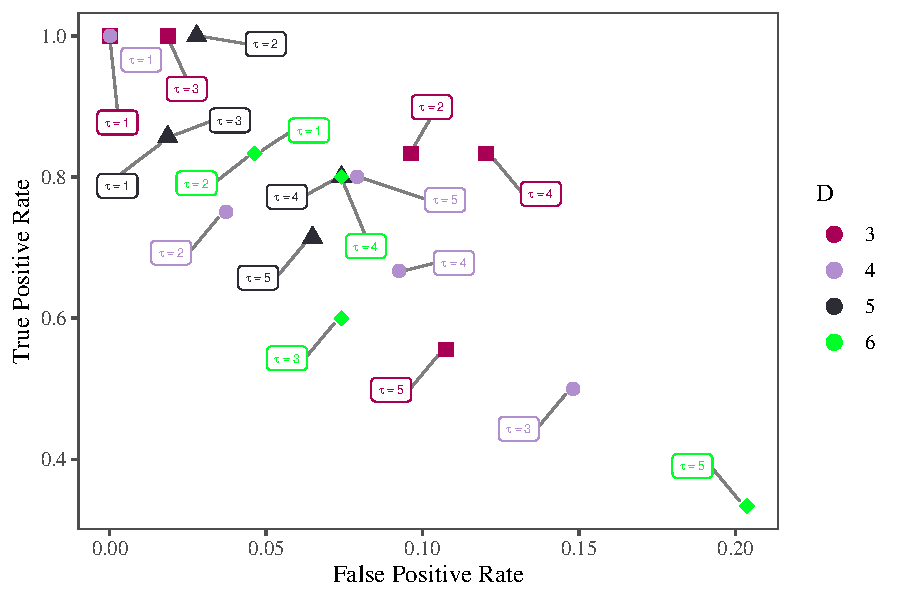
\includegraphics[width=\columnwidth]{Figures/ROC.pdf}
	\caption{Evaluation of the sliding window parameters using ROC curve}
	\label{fig:ROC}
\end{figure} 

We used the ROC curve shown in Fig.~\ref{fig:ROC} for different values of $D \in \{3, 4, 5, 6 \} $ and $\tau \in \{1, 2, 3, 4, 5 \}$ to select the best configuration.
As we can see in Fig.~\ref{fig:ROC}, the configurations that extracted most information from the 1-D signal and, thus, that presented the best results in the experiments, are $(D = 3, \tau = 1)$ and $(D = 4, \tau = 1)$.
The technique, thus, shows its best performance choosing the parameters with the lowest computational cost.

Figure~\ref{fig:Regions} shows the points in the $H\times C$ produced by the same samples with all the parameters mentioned above.
The spatial distribution of the points changes with the parameters,
and certain configurations promote better separation.
This figure shows that discrimination ability decreases with increasing $\tau$.
Larger values of delay dilute the spatial dependence, as neighboring points in the sample tend to be more distant in the image.
For this reason, we will use $\tau=1$.
Considering $\tau=1$ (first column of Fig.~\ref{fig:Regions}), 
we also notice that $D=3$ produces the best separation among classes.
Increasing $D$ also increases the Statistical Complexity; this is noticeable for the Forest class.
The other effect of considering larger values of $D$ is an increased Entropy of Ocean and, with it, an undesirable overlap with Urban samples.

\begin{sidewaysfigure*}
	\centering
	
\includegraphics[width=1\textwidth]{Figures/WATGHC.pdf}
	\caption{Characterization resulting in $H \times C$ Plane from the application of the Hilbert-Peano curve in WATG on textures of different regions: Guatemala (forest), Cape Canaveral (ocean) and Munich (urban). 
	The continuous curves correspond to the maximum and minimum values of $C$ as a function of $H$.}
	\label{fig:Regions}
\end{sidewaysfigure*}

\subsection{Quantitative Evaluation}

We present a comparison between our proposal and other methods for characterization and texture classification.
We use the following ten methods: 
Gabor filters~\cite{weldon1996efficient},  
Histogram of oriented gradients (HOG)~\cite{dalal2005histograms},
Gray-level co-occurrence matrices (GLCM)~\cite{kourgli2012texture}, 
Speeded-Up Robust Features (SURF)~\cite{bay2006surf},
Short Time Fourier Transform (STFT)~\cite{portnoff1980time} with SURF,
Bandt-Pompe probability distribution~\cite{Bandt2002Permutation}, 
Ordinal patterns transition graphs~\cite{Borges2019Transition},
Weighted Permutation Entropy (WPE)~\cite{Fadlallah2013Weightedpermutation},
Fine-Grained Permutation Entropy (FGPE)~\cite{xiao2009fine} with $\alpha = 0.5$, and
Amplitude-Aware Permutation Entropy (AAPE)~\cite{azami2016amplitude} with $A = 0.5$.
As in~\cite{guan2019covariance}, 
we computed four statistics from co-occurrence matrices: contrast, correlation, energy, and homogeneity.
Likewise, we implemented the Gabor filters in five scales and eight orientations; using the energy, we obtained an $80$-dimensional feature vector for each patch.
For the HOG technique, we used image pixels divided into cells equal to $3 \times 3$ pixels, where for each cell 6-bin histograms ranging from $0$ to $180$ degrees or $0$ to $360$ degrees.

In the classification, we used the $k$-nearest neighbor algorithm with Euclidean distance, selecting the value of $k$ with the automatic grid search method of the Caret R package~\cite{kuhn2008building}.
%In the following, we used $k = 20$.
For validation, we used $10$-fold cross-validation.
More details about the classifier and the sampling can be seen in~\cite{mitchell1997machine}.

Table~\ref{tab:result1} summarizes the number of features each method produces, as well as its performance of classifying the $200$ samples.
We assess the effectiveness of each approach using the following metrics: 
\begin{itemize}
	\item Recall or True Positive Rate (TPR): Total of the correctly detected class of regions over the total of regions for given ground truth.
	\begin{equation*}
	TPR = \frac{\text{True Positive}}{\text{True Positive} + \text{False Negative}}.
	\end{equation*}
	\item Precision or Positive Predictive Value (PPV): Total of regions correctly predicted over the total of regions classified by the algorithm.
	\begin{equation*}
	PPV = \frac{\text{True Positive}}{\text{True Positive} + \text{False Positive}}.
	\end{equation*}
	\item Overall Accuracy (OA): Total of regions correctly classified. 
	Knowing the number of true positive (TP) for each region, we have to:
	\begin{equation*}
	OA = \frac{\text{TP}_{ocean} + \text{TP}_{forest} + \text{TP}_{urban}}{\text{Total Regions}}.
	\end{equation*}
<<<<<<< HEAD
	The robustness analysis in image rotations was performed using $I(l)^T$, which corresponds to the $I$ transpose.
	Examples of the different images generated can be seen in Fig.~\ref{fig:speckle}.
	
	\begin{figure}[hbt]
		\begin{tabular}{ccc}
			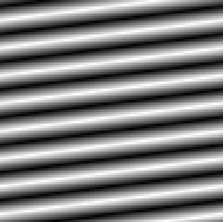
\includegraphics[width=0.135\textwidth]{Figures/z.png} &   
			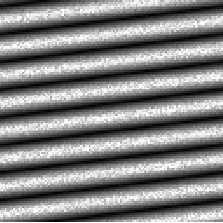
\includegraphics[width=0.135\textwidth]{Figures/z100.png} &
			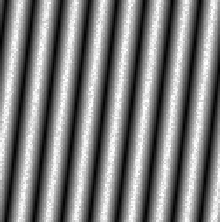
\includegraphics[width=0.135\textwidth]{Figures/z500t.png} \\
			(a) $z$ &   
			(b) $I(100)$ &
			(c) $I^T(500)$ \\
		\end{tabular}
		\caption{Visual representation of the data used in the robustness experiment.}
		\label{fig:speckle}
	\end{figure}

    As a result, we were able to verify that the higher $I$, the less noisy the pixels become, and we can see the in Fig.~\Ref{fig:speckleHC} that the statistical complexity and permutation entropy of the associated texture will be lower.
    On the other hand, we observe that the features are slightly sensitive to rotation, presenting variations in the order of magnitude of only 4 decimal places, thus maintaining the order of the position of the samples in the $H \times C$ plane.
    
	\begin{figure}[hbt]
		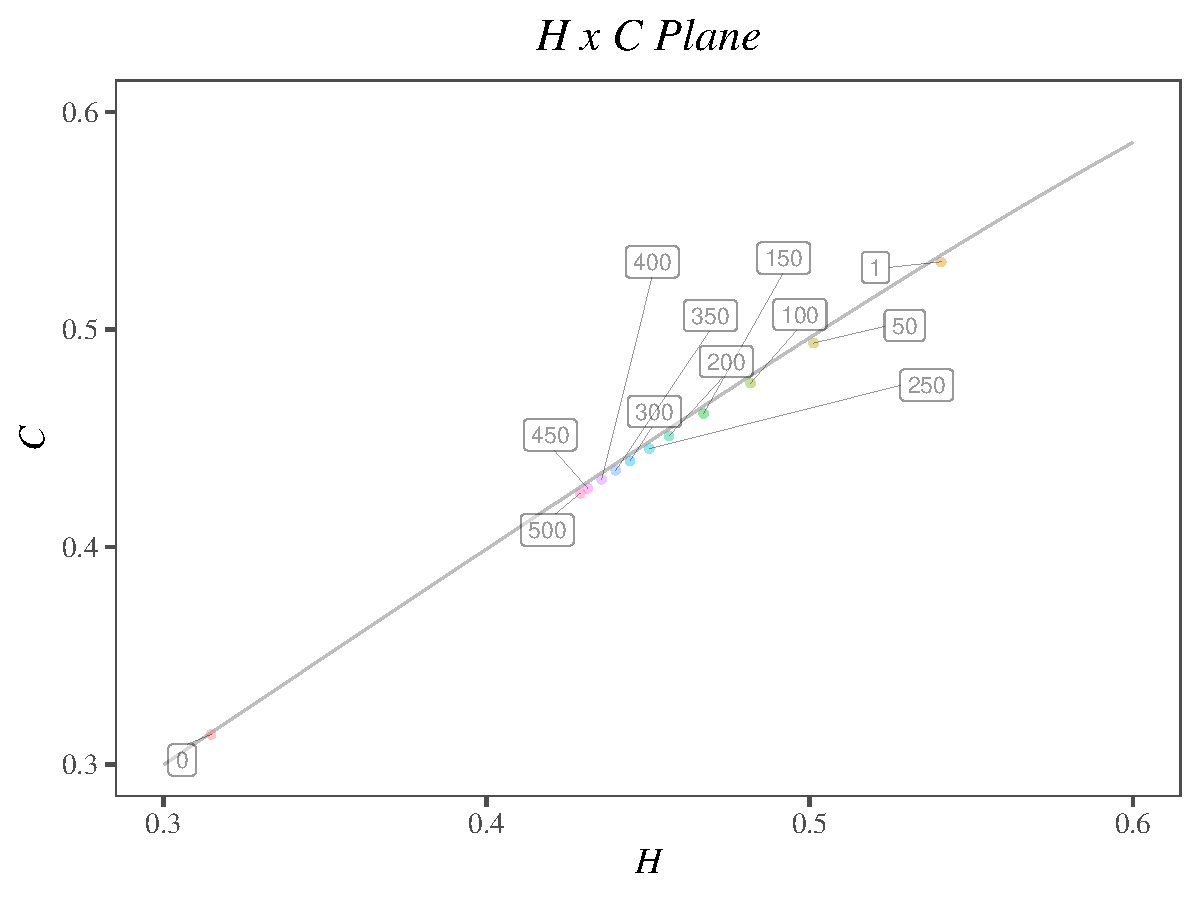
\includegraphics[width=0.45\textwidth]{Figures/waves1.pdf}
		\caption{Modifications to the $H \times C$ Plane features for $D = 6$ and $\tau = 1$ by adding different multiplicative noises.
        The continuous curves correspond to the maximum and minimum values of $C$ as a function of $H$.}
		\label{fig:speckleHC}
	\end{figure}

	\section{EXPERIMENTAL RESULTS AND ANALYSIS}\label{Results}
	
	In this section, we describe the dataset, 
	the classification process, and 
	the results of the experiments.
	To assess the performance of the technique here proposed, we first analyze the impact of its parameters and then compare its results in the classification with other methods.
	
	\subsection{Image Dataset}
	
	The proposed method was evaluated by dataset based on three quad-polarimetric L-band SAR images from the NASA Jet Propulsion Laboratory’s (JPL’s) uninhabited aerial vehicle synthetic aperture radar (UAVSAR) with $\sim 2$m range resolution and $36$ looks.
	We used the HH backscatter magnitudes of:
	\begin{itemize}
		\item Sierra del Lacandón National Park, forest region in Guatemala (acquired on April 10, 2015)\footnote{\protect{\url{https://uavsar.jpl.nasa.gov/cgi-bin/product.pl?jobName=Lacand_30202_15043_006_150410_L090_CX_01\#dados}}}. 
		It was $8917 \times 3300$ pixels and its image resolution is $10$m $\times 2$m;
		\item Cape Canaveral Ocean Regions (acquired on September 22, 2016).
		It was $7038 \times 3300$ pixels and its image resolution is $10$m $\times 2$m;
		\item Urban area of the city of Munich, Germany (acquired on June 5, 2015)\footnote{\protect{\url{https://uavsar.jpl.nasa.gov/cgi-bin/product.pl?jobName=munich_19417_15088_002_150605_L090_CX_01\#data}}}.
		It was $5773 \times 3300$ pixels and its image resolution is $10$m $\times 3$m.
	\end{itemize}
	
	We manually selected $200$ samples of size $128 \times 128$ to compose the dataset used in the experiments.
	It is organized as follows:
	$40$ samples from Guatemalan forest regions;
	$40$ samples from Guatemalan pasture regions;
	$80$ samples from the oceanic regions of Cape Canaveral, divided into two types with different contrast; and
	$40$ samples of urban regions of the city of Munich.
	Fig.~\ref{fig:samples} shows examples of each.
	
	%In the classification, to avoid overlapping between samples and to preserve the general distribution of the classes, the training, test and validation data were determined based on a random sampling carried out in each region of analysis.
	We randomly split the samples in training (\SI{85}{\percent}) and test (\SI{15}{\percent}) sets.
	We used the first set to train a $k$-nearest neighbor classifier algorithm with tenfold cross-validation.
	%The test samples were not used in the training stage.
	
	\subsection{Analysis of ordinal patterns methods}
	
	Fig.~\ref{fig:timeSeries} shows examples of the ocean, forest, urban, and pasture samples as sequences values, after the linearization process.
	Data resulting from remote sensing have a peculiar feature that justifies the application in this article:
	The variation in the magnitude of the targets' backscatter and, consequently, in the intensity of the image pixels, depends on the intrinsic properties of the regions under analysis.
	Urban targets usually exhibit the strongest variation, followed by pasture, forests, and finally, water bodies.
	By adding information related to amplitude, the proposed method is able to increase, compared to traditional methods, the granularity of information captured by ordinal patterns.
	Fig.~\ref{fig:plotsHC} shows the evolution of the descriptive power of these techniques.
	
	The Bandt-Pompe symbolization was the first method based on ordinal patterns proposed in the literature.
	As shown in Fig.~\ref{fig:plotsHC} left, it provides a limited separation of the textures.
	Transition graphs (Fig.~\ref{fig:plotsHC} center) improve the spread of the features, but with some amount of confusion.
	Our proposal, shown in Fig.~\ref{fig:plotsHC} right, produces well-separated features.
	%When considering the dynamics of alternating between consecutive patterns in a sequence, the transition graphs provide more information about the reference target and, consequently, this method is able to differentiate most of these dynamics, but there are challenging situations without a clear separation between them, causing misclassifications.
	%On the other hand, as discussed in the section~\ref{WATG}, the weighted graph provides greater weight for transitions between ordinal patterns that have a wide range of amplitude.
	%While in the traditional graph, the weight of the edges was obtained only by the frequency of the transitions, in the proposed method the symbols that appear with the same frequency gain different importance.
	In this way, we were able to obtain, for this experiment, a perfect characterization and, consequently, the high descriptive power of the regions.
	%In addition, some edges may disappear if the variation in amplitude between ordinal patterns is zero.
	
	\begin{figure*}[hbt]
		\begin{tabular}{ccccc}
			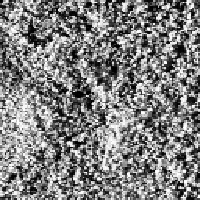
\includegraphics[width=0.175\textwidth]{Figures/guatemalaflorest.pdf} &   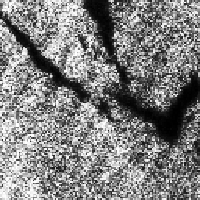
\includegraphics[width=0.175\textwidth]{Figures/Cape1.pdf} &
			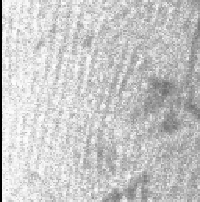
\includegraphics[width=0.175\textwidth]{Figures/Cape2.pdf} &  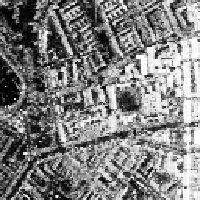
\includegraphics[width=0.175\textwidth]{Figures/munichUrban.pdf} &  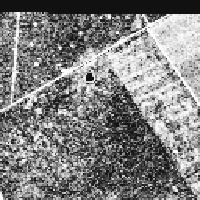
\includegraphics[width=0.175\textwidth]{Figures/pasture.pdf} \\
		\end{tabular}
		\caption{Types of regions analyzed: Guatemala forest, Canaveral ocean type 1, ocean type 2, Munich urban area, and pasture area.}
		\label{fig:samples}
	\end{figure*}
	
	\begin{figure*}[hbt]
		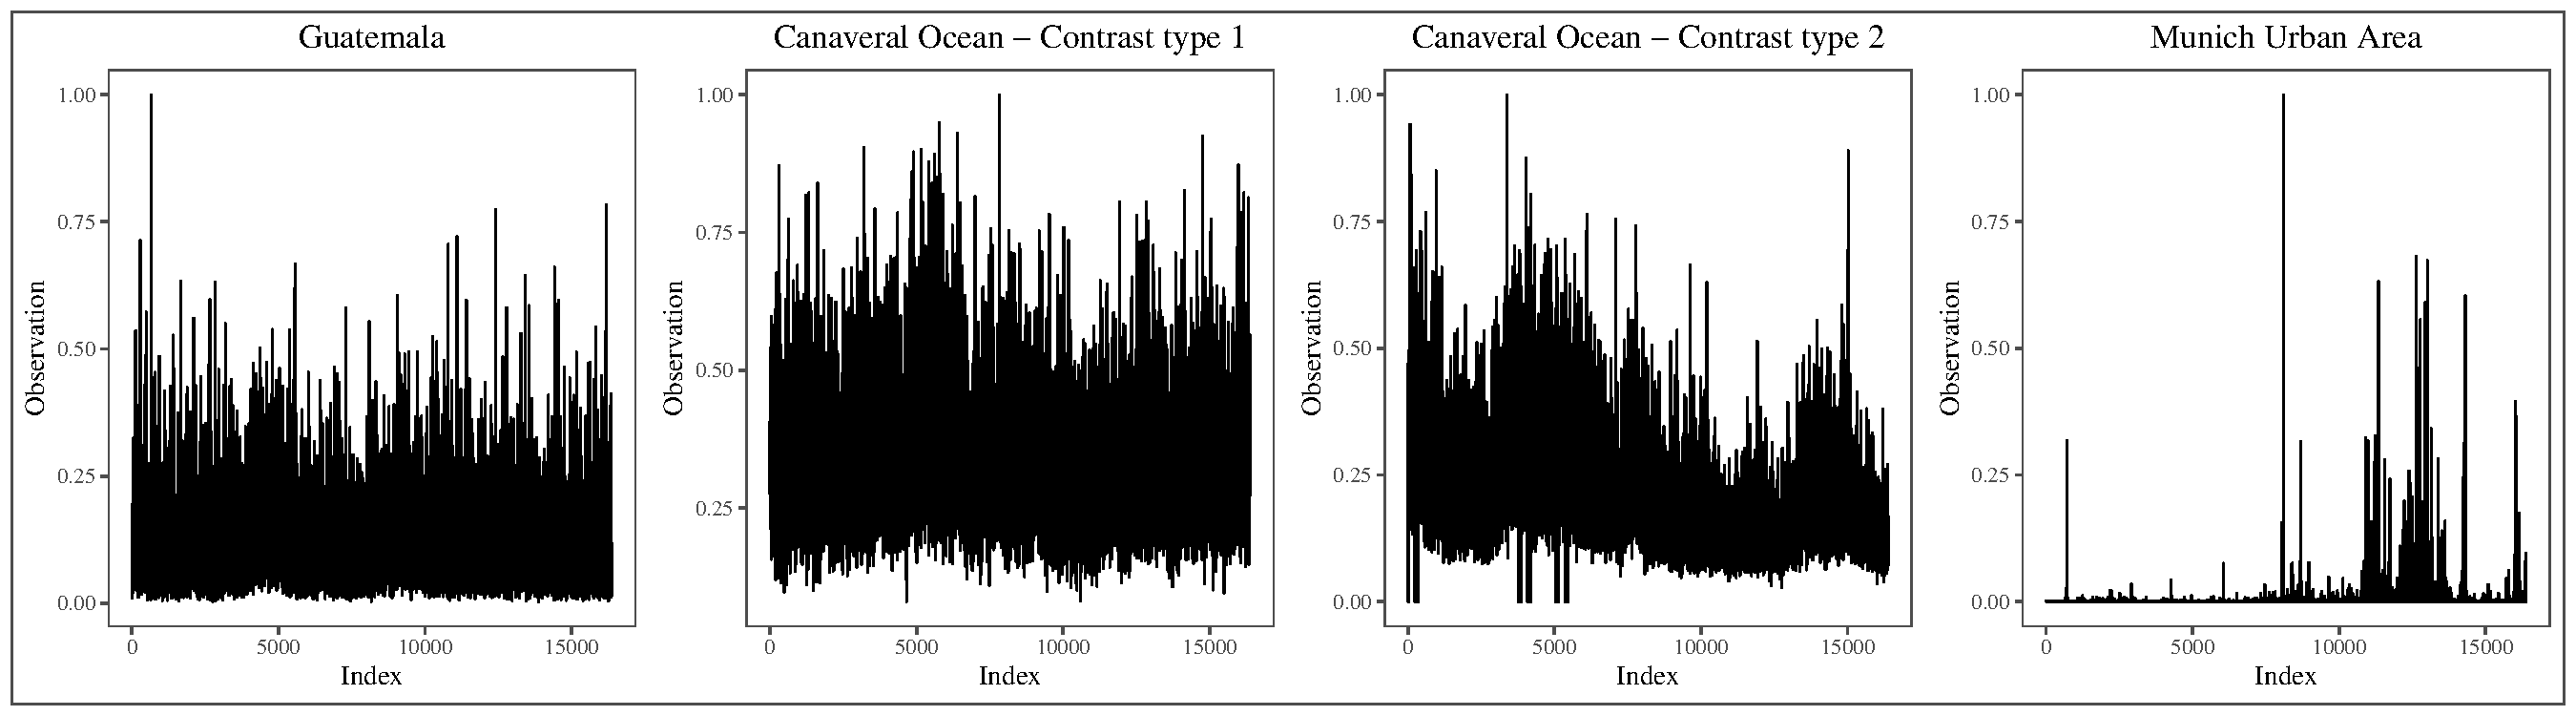
\includegraphics[width=2\columnwidth]{Figures/SAR_TS.pdf}
		\caption{Amplitude of different types of regions}
		\label{fig:timeSeries}
	\end{figure*}
	
	\begin{figure*}[hbt]
		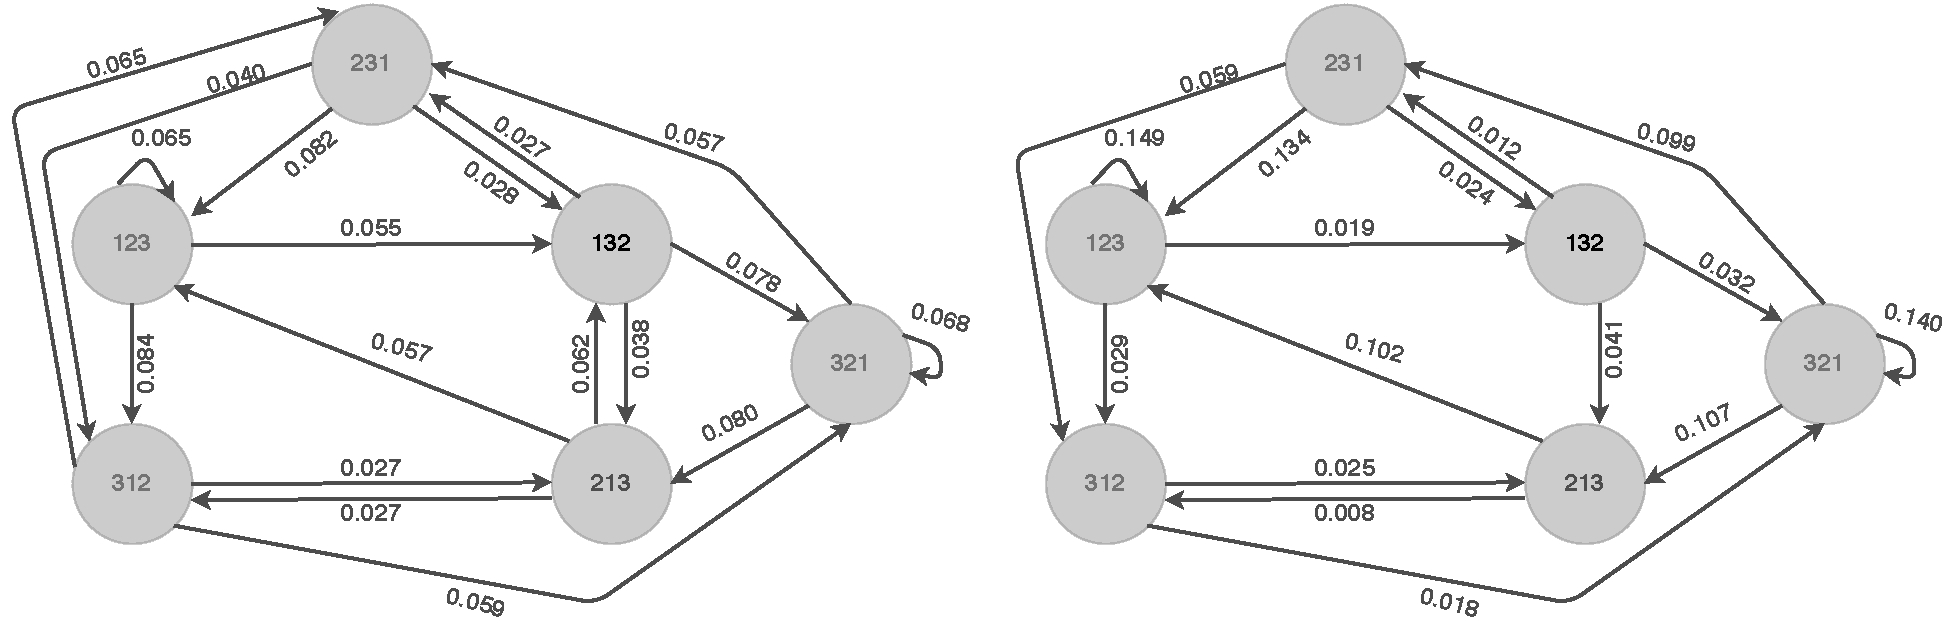
\includegraphics[width=2\columnwidth]{Figures/graphs.pdf}
		\caption{Example of the difference in weights at the edges in a sample of Munich urban regions in the transition graph and in the weighted graph of ordinal patterns
			transition to dimension 3 and delay 1}
		\label{fig:graphs}
	\end{figure*}
	
	\begin{figure*}[hbt]
		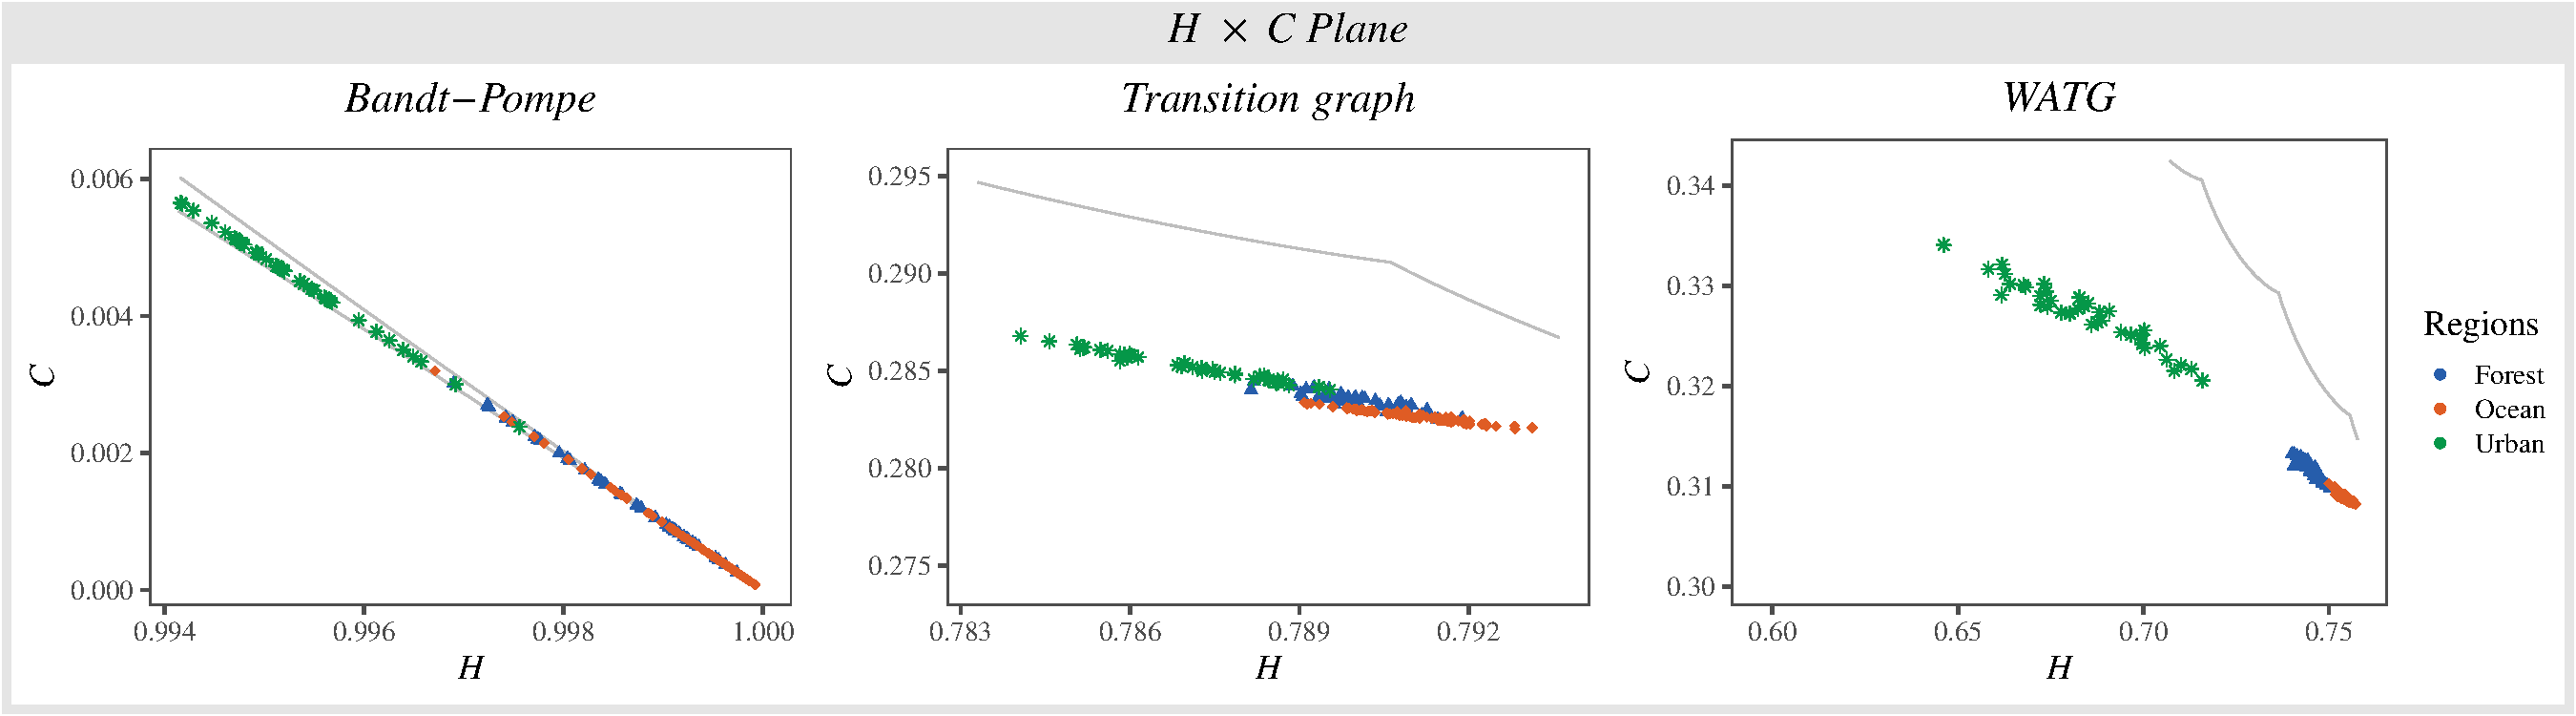
\includegraphics[width=2\columnwidth]{Figures/HCAnalysis.pdf}
		\caption{Location of Guatemala (forest), Cape Canaveral (ocean), and Munich (urban) in the $H \times C$ plane for dimension 3 and delay 1. 
			The continuous curves correspond to the maximum and minimum values of $C$ as a function of $H$.}
		\label{fig:plotsHC}
	\end{figure*}
	
	As already described in Section~\ref{WATG}, our proposal weights the edges in terms of the difference of amplitudes.
	As expected, the greatest impact is observed on the transition graphs obtained from urban areas.
	The urban area 1-D signal shown in Fig.~\ref{fig:timeSeries} has the largest dynamic range.
	Fig.~\ref{fig:graphs} shows how this information alters the weights of the transition graph.
	Notice, in particular, that 
	$(v_{\widetilde \pi^3_{123}}, v_{\widetilde \pi^3_{123}})$ almost doubled, while 
	$(v_{\widetilde \pi^3_{312}}, v_{\widetilde \pi^3_{231}})$ and $(v_{\widetilde \pi^3_{213}}, v_{\widetilde \pi^3_{132}})$ became negligible.
	We highlight the impact of the weighting on the probability distribution in the two extreme cases observed:
	\begin{itemize}
		\item If the 1-D signal presents a low amplitude variation and intensity peaks between, then the transitions of ordinal patterns that represent the latter have larger weights.
		This contributes so that the probability distribution becomes less uniform among the symbols, since it will be more concentrated in these edges.
		This will also cause a drop in the Entropy, when compared to the traditional method.
		\item In 1-D signal that show a uniform amplitude variation, the weights are well distributed between their edges, giving rise to a more random probability distribution, thus obtaining larger entropy.
	\end{itemize}
	
	\subsection{Experiments on sliding window selection}
	
	In this section, we analyze the parameters of the proposed method and its impact on the classification of textures.
	McCullough et al.~\cite{McCullough2015lagged} report that inadequate values may hinder important characteristics of the phenomenon under analysis.
	The two parameters of the transition graph are the dimension $D$, and the delay $\tau$.
	In the experiments below, we present the results in the classification using different values of these parameters.
	
	The performance of the classification method based on ordinal patterns is sensitive to window size, the embedding dimension, and the delay.
	In techniques based in Bandt-Pompe symbolization, for a fixed time series, as the size of embedding dimension decreases, more ordinal patterns are produced.
	Therefore, we acquire a greater granularity of information about the dynamics of the system and, consequently, we capture more spatial dependencies between the elements.
	
	\begin{figure}[hbt]
		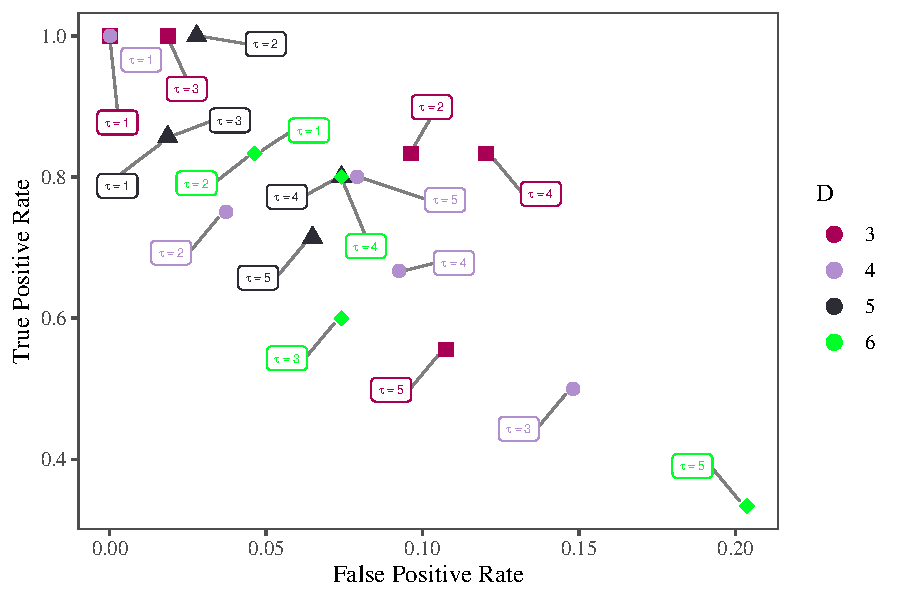
\includegraphics[width=\columnwidth]{Figures/ROC.pdf}
		\caption{Evaluation of the sliding window parameters using ROC curve}
		\label{fig:ROC}
	\end{figure} 
	
	We used the ROC curve shown in Fig.~\ref{fig:ROC} for different values of $D \in \{3, 4, 5, 6 \} $ and $\tau \in \{1, 2, 3, 4, 5 \}$ to select the best configuration.
	As we can see in Fig.~\ref{fig:ROC}, the configurations that extracted most information from the 1-D signal and, thus, that presented the best results in the experiments, are $(D = 3, \tau = 1)$ and $(D = 4, \tau = 1)$.
	The technique, thus, shows its best performance choosing the parameters with the lowest computational cost.
	
	Figure~\ref{fig:Regions} shows the points in the $H\times C$ produced by the same samples with all the parameters mentioned above.
	The spatial distribution of the points changes with the parameters,
	and certain configurations promote better separation.
	This figure shows that discrimination ability decreases with increasing $\tau$.
	Larger values of delay dilute the spatial dependence, as neighboring points in the sample tend to be more distant in the image.
	For this reason, we will use $\tau=1$.
	Considering $\tau=1$ (first column of Fig.~\ref{fig:Regions}), 
	we also notice that $D=3$ produces the best separation among classes.
	Increasing $D$ also increases the Statistical Complexity; this is noticeable for the Forest class.
	The other effect of considering larger values of $D$ is an increased Entropy of Ocean and, with it, an undesirable overlap with Urban samples.
	
	\begin{sidewaysfigure*}
		\centering
		
\includegraphics[width=1\textwidth]{Figures/WATGHC.pdf}
		\caption{Characterization resulting in $H \times C$ Plane from the application of the Hilbert-Peano curve in WATG on textures of different regions: Guatemala (forest), Cape Canaveral (ocean) and Munich (urban). 
		The continuous curves correspond to the maximum and minimum values of $C$ as a function of $H$.}
		\label{fig:Regions}
	\end{sidewaysfigure*}
	
	\subsection{Quantitative Evaluation}
	
	We present a comparison between our proposal and other methods for characterization and texture classification.
    We use the following ten methods: 
	Gabor filters~\cite{weldon1996efficient},  
    Histogram of oriented gradients (HOG)~\cite{dalal2005histograms},
	Gray-level co-occurrence matrices (GLCM)~\cite{kourgli2012texture}, 
    Speeded-Up Robust Features (SURF)~\cite{bay2006surf},
    Short Time Fourier Transform (STFT)~\cite{portnoff1980time} with SURF,
	Bandt-Pompe probability distribution~\cite{Bandt2002Permutation}, 
	Ordinal patterns transition graphs~\cite{Borges2019Transition},
	Weighted Permutation Entropy (WPE)~\cite{Fadlallah2013Weightedpermutation},
	Fine-Grained Permutation Entropy (FGPE)~\cite{xiao2009fine} with $\alpha = 0.5$, and
	Amplitude-Aware Permutation Entropy (AAPE)~\cite{azami2016amplitude} with $A = 0.5$.
	As in~\cite{guan2019covariance}, 
    we computed four statistics from co-occurrence matrices: contrast, correlation, energy, and homogeneity.
    Likewise, we implemented the Gabor filters in five scales and eight orientations; using the energy, we obtained an $80$-dimensional feature vector for each patch.
    For the HOG technique, we used image pixels divided into cells equal to $3 \times 3$ pixels, where for each cell 6-bin histograms ranging from $0$ to $180$ degrees or $0$ to $360$ degrees.
	
	In the classification, we used the $k$-nearest neighbor algorithm with Euclidean distance, selecting the value of $k$ with the automatic grid search method of the Caret R package~\cite{kuhn2008building}.
	%In the following, we used $k = 20$.
	For validation, we used $10$-fold cross-validation.
	More details about the classifier and the sampling can be seen in~\cite{mitchell1997machine}.
	
	Table~\ref{tab:result1} summarizes the number of features each method produces, as well as its performance of classifying the $200$ samples.
	We assess the effectiveness of each approach using the following metrics: 
	\begin{itemize}
		\item Recall or True Positive Rate (TPR): Total of the correctly detected class of regions over the total of regions for given ground truth.
		\begin{equation*}
		TPR = \frac{\text{True Positive}}{\text{True Positive} + \text{False Negative}}.
		\end{equation*}
		\item Precision or Positive Predictive Value (PPV): Total of regions correctly predicted over the total of regions classified by the algorithm.
		\begin{equation*}
		PPV = \frac{\text{True Positive}}{\text{True Positive} + \text{False Positive}}.
		\end{equation*}
		\item Overall Accuracy (OA): Total of regions correctly classified. 
		Knowing the number of true positive (TP) for each region, we have to:
		\begin{equation*}
		OA = \frac{\text{TP}_{ocean} + \text{TP}_{forest} + \text{TP}_{urban}}{\text{Total Regions}}.
		\end{equation*}
		\item F1-score: The harmonic mean of precision and recall.
		\begin{equation*}
		\text{F1-score} = 2 \times \frac{PPV \times TPR}{PPV + TPR}.
		\end{equation*}
	\end{itemize}
	
	\begin{table*}[hbt]
		\centering
		\caption{Experimental results using $k$-NN}
		\label{tab:result1}
		\begin{tabular}{lrrr*9{r}}
			\toprule
			\multirow{2}{*}{Method} & \multirow{2}{*}{\# features} & & TPR & & & & PPV & & & \multirow{2}{*}{OA} & \multirow{2}{*}{F1-Score} \\ 
			\cmidrule(lr){3-6} 
			\cmidrule(lr){7-10}
			&   & Forest & Pasture & Ocean & Urban & Forest & Pasture & Ocean & Urban & &  \\ 
			\cmidrule(lr){1-1}
			\cmidrule(lr){2-2}
			\cmidrule(lr){3-6}
			\cmidrule(lr){7-10}
			\cmidrule(lr){11-11}
			\cmidrule(lr){12-12}
			Gabor & 80 & 
			1.000 & 1.000 & 1.000 & 1.000 & 
			1.000 & 1.000 & 1.000 & 1.000 & 
			1.000 & 1.000\\
			HOG & 54 & 
			1.000 & 1.000 & 1.000 & 1.000 & 
			1.000 & 1.000 & 1.000 & 1.000 & 
			1.000 & 1.000\\
			GLCM & 32 & 
			0.833 & 1.000 & 1.000 & 0.833 &
			1.000 & 0.857 & 0.923 & 1.000 &
			0.933 & 0.909\\
			SURF & 1856 & 
			0.500 & 0.000 & 1.000 & 0.000 & 
			1.000 & 0.000 & 0.444 & 0.000 &
			0.500 & 0.666\\
			STFT + SURF  & 1856 & 
			0.166 & 0.000 & 0.833 & 0.166 & 
			0.250 & 0.000 & 0.416 & 0.500 &
			0.400 & 0.200\\
			\cmidrule(lr){1-1}
			\cmidrule(lr){2-2}
			\cmidrule(lr){3-6}
			\cmidrule(lr){7-10}
			\cmidrule(lr){11-11}
			\cmidrule(lr){12-12}
			Bandt-Pompe & 2 & 
			0.333 & 1.000 & 0.750 & 1.000 &
			0.500 & 0.857 & 0.750 & 0.857 &
			0.766 & 0.400\\ 
			Transition Graph & 2 & 
			0.833 & 0.666 & 0.833 & 1.000 &
			0.833 & 0.800 & 0.769 & 1.000 &
			0.833 & 0.833\\
			\cmidrule(lr){1-1}
			\cmidrule(lr){2-2}
			\cmidrule(lr){3-6}
			\cmidrule(lr){7-10}
			\cmidrule(lr){11-11}
			\cmidrule(lr){12-12}
			WPE & 2 & 
			1.000 & 0.833 & 1.000 & 0.833 &
			0.857 & 0.833 & 1.000 & 1.000 &
			0.933 & 0.923\\ 
			AAPE & 2 & 
			0.666 & 1.000 & 1.000 & 1.000 &
			1.000 & 0.857 & 0.923 & 1.000 &
			0.933 & 0.800\\ 
			FGPE & 2 & 
			0.666 & 0.666 & 1.000 & 1.000 &
			0.800 & 0.666 & 0.923 & 1.000 &
			0.866 & 0.727\\ 
			\cmidrule(lr){1-1}
			\cmidrule(lr){2-2}
			\cmidrule(lr){3-6}
			\cmidrule(lr){7-10}
			\cmidrule(lr){11-11}
			\cmidrule(lr){12-12}
			WATG & 2 & 
			1.000 & 1.000 & 1.000 & 1.000 &
			1.000 & 1.000 & 1.000 & 1.000 &
			1.000 & 1.000\\
			\bottomrule
		\end{tabular}
	\end{table*}
	
	As we can observed in Table~\ref{tab:result1}, among the methods of weighting ordinal patterns, FGPE produced the worst results: $\text{OA}=\SI{86.6}{\percent}$ and $\text{F1-score}=\SI{72.7}{\percent}$.
	%
	AAPE also produced a low F1-score result, but it produced more consistent results in the other metrics, presenting $\text{OA} = \SI{93.3}{\percent}$.
	%
	On the other hand, WPE achieved one of the best results of the developed analysis: $\text{OA}=\SI{93.3}{\percent}$ and $\text{F1-score}=\SI{92.3}{\percent}$.
	%
	Therefore, we found that among such methods, WATG is the one that best describes the textures presented, obtaining the best performance.
	
	
	The STFT + SURF produced the worst results: $\text{OA}=\SI{40.0}{\percent}$ and $\text{F1-score}=\SI{20.0}{\percent}$.
	%
    On the other hand, the application of the SURF descriptor alone provided a better performance:  $\text{OA}=\SI{50.0}{\percent}$ and $\text{F1-score}=\SI{66.6}{\percent}$.
	%
    Since the problem analyzed consists of classification with few samples, although the classification method GLCM-based obtains good TPR and PPV, it has a low OA provided by the impact of the presence of false-positive and false-negative results.
    %
	%Bandt-Pompe improve these classification results, leading to  %$\text{OA}=\SI{79.1}{\percent}$ and %$\text{F1-score}=\SI{54.5}{\percent}$.
	%
	Among all handcraft methods analyzed, HOG and Gabor filters achievement the highest success rate in the classification tasks with $\text{OA} = \SI{100}{\percent}$ and $\text{F1-score} = \SI{100}{\percent}$.
    However, WATG achieves that same performance using only $2$ features.
    This reduction implies less computational power requirement and avoids the curse of dimensionality~\cite{TheCursesofDimensionality2018}.
	
	\section{CONCLUSION}\label{Conclusion}
	
	We presented and assessed a new method of analysis and classification of SAR image textures.
	This method consists of three steps: 
	(1)~linearization, 
	(2)~computing the Weighted Ordinal Pattern Transition Graph, and 
	(3)~obtaining Information Theory descriptors.	
	With the use of the WATG technique, we can find a probability distribution function of ordinal patterns that is sensitive to amplitude information and then apply the $k$-NN algorithm to classify the descriptors.
	As a result, in addition to perfectly separating urban areas and pasture from the others analyzed by entropy values, we are still able to differentiate oceanic and forest areas through their different values of statistical complexity, which informs us of the degree of spatial dependence between their elements.
	
	Experiments using patches from UAVSAR images showed that the proposal performs better than GLCM, Bandt-Pompe, Transition Graphs, SURF, STFT + SURF, and other techniques of amplitude information analysis in ordinal patterns and that it provides the same quality of results obtained with Gabor filters and HOG.
	However, while Gabor filters employ $80$ features and HOG employ $54$ features, our proposal requires only two.
	Since the proposed method has a lower number of descriptive features than its direct competitors, we were able to obtain some additional advantages under this.
	First, by reducing the dimension of the features to 2-D, we can accurately visualize the differences between the classes of regions analyzed.
	In addition, for machine learning algorithms, the smaller the number of dimensions, the faster the process, and less storage space are required.
	So, we managed to avoid overfitting classification models, a recurring problem in data with high dimensionality.
	
	Since the application of this work is limited to texture patches from homogeneous regions, we aim in the future study the possible impacts of analysis on heterogeneous areas, such as cultivation zones and mixed urban regions.
	The use of transition detection techniques and the segmentation of these signals in a stage before the use of WATG may increase the power of its application and will be fruitful avenues for future work.
	
	
	\section{SOURCE CODE AVAILABILITY} 
	
	The text, source code, and data used in this study are available at the \textit{SAR-WATG} repository \url{https://github.com/EduardaChagas/SAR-WATG}.
	
	\bibliographystyle{IEEEtran}
	%\bibliography{bibtex/sar.bib}
	\bibliography{AbbrevRefs}
	
	\section*{ACKNOWLEDGEMENTS}\label{ACKNOWLEDGEMENTS}
	
	This work was partially funded by the Coordination for the Improvement of Higher Education Personnel (CAPES) and National Council for Scientific and Technological Development (CNPq).
	
=======
	\item F1-score: The harmonic mean of precision and recall.
	\begin{equation*}
	\text{F1-score} = 2 \times \frac{PPV \times TPR}{PPV + TPR}.
	\end{equation*}
\end{itemize}

\begin{table*}[hbt]
	\centering
	\caption{Experimental results using $k$-NN}
	\label{tab:result1}
	\begin{tabular}{lrrr*9{r}}
		\toprule
		\multirow{2}{*}{Method} & \multirow{2}{*}{\# features} & & TPR & & & & PPV & & & \multirow{2}{*}{OA} & \multirow{2}{*}{F1-Score} \\ 
		\cmidrule(lr){3-6} 
		\cmidrule(lr){7-10}
		&   & Forest & Pasture & Ocean & Urban & Forest & Pasture & Ocean & Urban & &  \\ 
		\cmidrule(lr){1-1}
		\cmidrule(lr){2-2}
		\cmidrule(lr){3-6}
		\cmidrule(lr){7-10}
		\cmidrule(lr){11-11}
		\cmidrule(lr){12-12}
		Gabor & 80 & 
		1.000 & 1.000 & 1.000 & 1.000 & 
		1.000 & 1.000 & 1.000 & 1.000 & 
		1.000 & 1.000\\
		HOG & 54 & 
		1.000 & 1.000 & 1.000 & 1.000 & 
		1.000 & 1.000 & 1.000 & 1.000 & 
		1.000 & 1.000\\
		GLCM & 32 & 
		0.833 & 1.000 & 1.000 & 0.833 &
		1.000 & 0.857 & 0.923 & 1.000 &
		0.933 & 0.909\\
		SURF & 1856 & 
		0.500 & 0.000 & 1.000 & 0.000 & 
		1.000 & 0.000 & 0.444 & 0.000 &
		0.500 & 0.666\\
		STFT + SURF  & 1856 & 
		0.166 & 0.000 & 0.833 & 0.166 & 
		0.250 & 0.000 & 0.416 & 0.500 &
		0.400 & 0.200\\
		\cmidrule(lr){1-1}
		\cmidrule(lr){2-2}
		\cmidrule(lr){3-6}
		\cmidrule(lr){7-10}
		\cmidrule(lr){11-11}
		\cmidrule(lr){12-12}
		Bandt-Pompe & 2 & 
		0.333 & 1.000 & 0.750 & 1.000 &
		0.500 & 0.857 & 0.750 & 0.857 &
		0.766 & 0.400\\ 
		Transition Graph & 2 & 
		0.833 & 0.666 & 0.833 & 1.000 &
		0.833 & 0.800 & 0.769 & 1.000 &
		0.833 & 0.833\\
		\cmidrule(lr){1-1}
		\cmidrule(lr){2-2}
		\cmidrule(lr){3-6}
		\cmidrule(lr){7-10}
		\cmidrule(lr){11-11}
		\cmidrule(lr){12-12}
		WPE & 2 & 
		1.000 & 0.833 & 1.000 & 0.833 &
		0.857 & 0.833 & 1.000 & 1.000 &
		0.933 & 0.923\\ 
		AAPE & 2 & 
		0.666 & 1.000 & 1.000 & 1.000 &
		1.000 & 0.857 & 0.923 & 1.000 &
		0.933 & 0.800\\ 
		FGPE & 2 & 
		0.666 & 0.666 & 1.000 & 1.000 &
		0.800 & 0.666 & 0.923 & 1.000 &
		0.866 & 0.727\\ 
		\cmidrule(lr){1-1}
		\cmidrule(lr){2-2}
		\cmidrule(lr){3-6}
		\cmidrule(lr){7-10}
		\cmidrule(lr){11-11}
		\cmidrule(lr){12-12}
		WATG & 2 & 
		1.000 & 1.000 & 1.000 & 1.000 &
		1.000 & 1.000 & 1.000 & 1.000 &
		1.000 & 1.000\\
		\bottomrule
	\end{tabular}
\end{table*}

As we can observed in Table~\ref{tab:result1}, among the methods of weighting ordinal patterns, FGPE produced the worst results: $\text{OA}=\SI{86.6}{\percent}$ and $\text{F1-score}=\SI{72.7}{\percent}$.
%
AAPE also produced a low F1-score result, but it produced more consistent results in the other metrics, presenting $\text{OA} = \SI{93.3}{\percent}$.
%
On the other hand, WPE achieved one of the best results of the developed analysis: $\text{OA}=\SI{93.3}{\percent}$ and $\text{F1-score}=\SI{92.3}{\percent}$.
%
Therefore, we found that among such methods, WATG is the one that best describes the textures presented, obtaining the best performance.


The STFT + SURF produced the worst results: $\text{OA}=\SI{40.0}{\percent}$ and $\text{F1-score}=\SI{20.0}{\percent}$.
%
On the other hand, the application of the SURF descriptor alone provided a better performance:  $\text{OA}=\SI{50.0}{\percent}$ and $\text{F1-score}=\SI{66.6}{\percent}$.
%
Since the problem analyzed consists of classification with few samples, although the classification method GLCM-based obtains good TPR and PPV, it has a low OA provided by the impact of the presence of false-positive and false-negative results.
%
%Bandt-Pompe improve these classification results, leading to  %$\text{OA}=\SI{79.1}{\percent}$ and %$\text{F1-score}=\SI{54.5}{\percent}$.
%
Among all handcraft methods analyzed, HOG and Gabor filters achievement the highest success rate in the classification tasks with $\text{OA} = \SI{100}{\percent}$ and $\text{F1-score} = \SI{100}{\percent}$.
However, WATG achieves that same performance using only $2$ features.
This reduction implies less computational power requirement and avoids the curse of dimensionality~\cite{TheCursesofDimensionality2018}.

\section{CONCLUSION}\label{Conclusion}

We presented and assessed a new method of analysis and classification of SAR image textures.
This method consists of three steps: 
(1)~linearization, 
(2)~computing the Weighted Ordinal Pattern Transition Graph, and 
(3)~obtaining Information Theory descriptors.	
With the use of the WATG technique, we can find a probability distribution function of ordinal patterns that is sensitive to amplitude information and then apply the $k$-NN algorithm to classify the descriptors.
As a result, in addition to perfectly separating urban areas and pasture from the others analyzed by entropy values, we are still able to differentiate oceanic and forest areas through their different values of statistical complexity, which informs us of the degree of spatial dependence between their elements.

Experiments using patches from UAVSAR images showed that the proposal performs better than GLCM, Bandt-Pompe, Transition Graphs, SURF, STFT + SURF, and other techniques of amplitude information analysis in ordinal patterns and that it provides the same quality of results obtained with Gabor filters and HOG.
However, while Gabor filters employ $80$ features and HOG employ $54$ features, our proposal requires only two.
Since the proposed method has a lower number of descriptive features than its direct competitors, we were able to obtain some additional advantages under this.
First, by reducing the dimension of the features to 2-D, we can accurately visualize the differences between the classes of regions analyzed.
In addition, for machine learning algorithms, the smaller the number of dimensions, the faster the process, and less storage space are required.
So, we managed to avoid overfitting classification models, a recurring problem in data with high dimensionality.

Since the application of this work is limited to texture patches from homogeneous regions, we aim in the future study the possible impacts of analysis on heterogeneous areas, such as cultivation zones and mixed urban regions.
The use of transition detection techniques and the segmentation of these signals in a stage before the use of WATG may increase the power of its application and will be fruitful avenues for future work.


\section{SOURCE CODE AVAILABILITY} 

The text, source code, and data used in this study are available at the \textit{SAR-WATG} repository \url{https://github.com/EduardaChagas/SAR-WATG}.

\bibliographystyle{IEEEtran}
%\bibliography{bibtex/sar.bib}
\bibliography{AbbrevRefs}

\section*{ACKNOWLEDGEMENTS}\label{ACKNOWLEDGEMENTS}

This work was partially funded by the Coordination for the Improvement of Higher Education Personnel (CAPES) and National Council for Scientific and Technological Development (CNPq).

>>>>>>> Avançando
\end{document}  
